% Options for packages loaded elsewhere
\PassOptionsToPackage{unicode}{hyperref}
\PassOptionsToPackage{hyphens}{url}
\PassOptionsToPackage{dvipsnames,svgnames,x11names}{xcolor}
%
\documentclass[
  12pt,
  french,
  12pt,a4paper]{article}
\title{Estimation en temps réel de la tendance-cycle : apport de l'utilisation des filtres asymétriques dans la détection des points de retournement}
\author{Alain Quartier-la-Tente}
\date{2022-03-17}

\usepackage{amsmath,amssymb}
\usepackage{lmodern}
\usepackage{iftex}
\ifPDFTeX
  \usepackage[T1]{fontenc}
  \usepackage[utf8]{inputenc}
  \usepackage{textcomp} % provide euro and other symbols
\else % if luatex or xetex
  \usepackage{unicode-math}
  \defaultfontfeatures{Scale=MatchLowercase}
  \defaultfontfeatures[\rmfamily]{Ligatures=TeX,Scale=1}
\fi
% Use upquote if available, for straight quotes in verbatim environments
\IfFileExists{upquote.sty}{\usepackage{upquote}}{}
\IfFileExists{microtype.sty}{% use microtype if available
  \usepackage[]{microtype}
  \UseMicrotypeSet[protrusion]{basicmath} % disable protrusion for tt fonts
}{}
\makeatletter
\@ifundefined{KOMAClassName}{% if non-KOMA class
  \IfFileExists{parskip.sty}{%
    \usepackage{parskip}
  }{% else
    \setlength{\parindent}{0pt}
    \setlength{\parskip}{6pt plus 2pt minus 1pt}}
}{% if KOMA class
  \KOMAoptions{parskip=half}}
\makeatother
\usepackage{xcolor}
\IfFileExists{xurl.sty}{\usepackage{xurl}}{} % add URL line breaks if available
\IfFileExists{bookmark.sty}{\usepackage{bookmark}}{\usepackage{hyperref}}
\hypersetup{
  pdftitle={Estimation en temps réel de la tendance-cycle : apport de l'utilisation des filtres asymétriques dans la détection des points de retournement},
  pdfauthor={Alain Quartier-la-Tente},
  pdflang={fr},
  colorlinks=true,
  linkcolor={Maroon},
  filecolor={Maroon},
  citecolor={Blue},
  urlcolor={blue},
  pdfcreator={LaTeX via pandoc}}
\urlstyle{same} % disable monospaced font for URLs
\usepackage[hmargin = 25mm, vmargin = 25mm]{geometry}
\usepackage{longtable,booktabs,array}
\usepackage{calc} % for calculating minipage widths
% Correct order of tables after \paragraph or \subparagraph
\usepackage{etoolbox}
\makeatletter
\patchcmd\longtable{\par}{\if@noskipsec\mbox{}\fi\par}{}{}
\makeatother
% Allow footnotes in longtable head/foot
\IfFileExists{footnotehyper.sty}{\usepackage{footnotehyper}}{\usepackage{footnote}}
\makesavenoteenv{longtable}
\usepackage{graphicx}
\makeatletter
\def\maxwidth{\ifdim\Gin@nat@width>\linewidth\linewidth\else\Gin@nat@width\fi}
\def\maxheight{\ifdim\Gin@nat@height>\textheight\textheight\else\Gin@nat@height\fi}
\makeatother
% Scale images if necessary, so that they will not overflow the page
% margins by default, and it is still possible to overwrite the defaults
% using explicit options in \includegraphics[width, height, ...]{}
\setkeys{Gin}{width=\maxwidth,height=\maxheight,keepaspectratio}
% Set default figure placement to htbp
\makeatletter
\def\fps@figure{htbp}
\makeatother
\setlength{\emergencystretch}{3em} % prevent overfull lines
\providecommand{\tightlist}{%
  \setlength{\itemsep}{0pt}\setlength{\parskip}{0pt}}
\setcounter{secnumdepth}{5}
%début contraintes ensae
\usepackage{pdfpages, setspace, mathptmx} %times roman
\usepackage{textpos}%pour textblock

% Début JMS
\makeatletter
\def\@maketitle{%
\thispagestyle{fancy}
\begin{center}

\includegraphics[width=15cm]{img/head_jms2022.png} 
\line(1,0){450}
\vspace{5mm}
\textbf{{\huge E}\Large stimation en temps réel de la tendance-cycle : apport de l’utilisation des filtres asymétriques dans la détection des points de retournement}
\end{center}

\begin{center}
\textit{Alain QUARTIER-LA-TENTE} \\
\vspace{2mm}
\textit{(*) Insee,  Département des études économiques (DEE), et  Laboratoire d'Économie et de Management de Nantes-Atlantique (LEMNA)}\\
\vspace{2mm}
\url{alain.quartier-la-tente@insee.fr} 
\end{center}

\vspace{5mm}
\small{{\bf Mots-clés.} séries temporelles,  tendance-cycle,  désaisonnalisation,  \emph{nowcasting}.}

\vspace{5mm}
\small{{\bf Domaines.} 10.2 Désaisonnalisation --- 10.3 Nowcasting.}

\begin{center}
\line(1,0){450}
\end{center}

\normalsize
}
\usepackage{fancyhdr} 
\pagestyle{fancy}

\renewcommand{\headrulewidth}{0pt}
\fancyhead[C]{} 
\fancyhead[L]{}
\fancyhead[R]{}

\renewcommand{\footrulewidth}{0pt}
\fancyfoot[C]{\footnotesize{$14^{es}$ Journées de méthodologie statistique de l'Insee (JMS) / Mars 2022 / PARIS}}
\fancyfoot[R]{\thepage}
%FIN JMS

\makeatother% cinsérer page de garde

\usepackage{stmaryrd}
\usepackage{multicol}
\usepackage{graphicx}
\usepackage{animate, dsfont, here, xspace}
%\usepackage{tikz}       
\usepackage{tikz,pgfplots}
 \pgfplotsset{compat=1.17}
%\includepdf[fitpaper=true, pages=-]{img/pdg.pdf}


\DeclareMathOperator{\e}{e}
\DeclareMathOperator{\Determinant}{det}
\renewcommand{\P}{\mathds{P}} %Apparement \P existe déjà ?
\newcommand\N{\mathds{N}}
\newcommand\Norm{\mathcal{N}}
\newcommand\R{\mathds{R}}
\newcommand\Z{\mathds{Z}}
\newcommand{\determinant}[1]{\Determinant\left(#1\right)}
%\newcommand\C{\mathds{C}}
%\newcommand\Z{\mathds{Z}}


\newcommand\1{\mathds{1}}
\newcommand{\E}[2][]{{\mathds{E}}_{#1}
  \def\temp{#2}\ifx\temp\empty
  \else
    \left[#2\right]
  \fi
}
\newcommand{\V}[2][]{{\mathds{V}}_{#1}
  \def\temp{#2}\ifx\temp\empty
  \else
    \left[#2\right]
  \fi
}
\newcommand\ud{\,\mathrm{d}}
\newcommand{\ps}[2]{\left\langle #1 \,,\, #2 \right\rangle}

% blocks
\usepackage{environ}
\usepackage[tikz]{bclogo}

\tikzstyle{titlestyle} =[draw=black!80,fill=black!20, text=black,
 right=10pt, rounded corners]
\mdfdefinestyle{symmaryboxstyle}{
	linecolor=black!80, backgroundcolor = black!5,
	skipabove=\baselineskip, innertopmargin=\baselineskip,
	innerbottommargin=\baselineskip,
	userdefinedwidth=\textwidth,
	middlelinewidth=1.2pt, roundcorner=5pt,
	skipabove={\dimexpr0.5\baselineskip+\topskip\relax},
	frametitleaboveskip=\dimexpr-\ht\strutbox\relax,
	innerlinewidth=0pt,
}
\newcounter{summarybox}
\NewEnviron{summary_box}[2][true]{%
\refstepcounter{summarybox} % on incrémente le compteur
\begin{mdframed}[style=symmaryboxstyle,
nobreak=#1,
frametitle={%
      \tikz[baseline=(current bounding box.east),outer sep=0pt]
      \node[titlestyle,anchor=east]
    {Encadré \thesummarybox{} --- #2};}
]
\vspace{-0.5em}
\BODY
\end{mdframed}
}

\usepackage{amsthm}
%\theoremstyle{remark}
\newtheorem*{remarque}{Remarque}

\usepackage{mathrsfs}
\usepackage{fontawesome5}

\usepackage[style=authoryear,uniquename=false, uniquelist=false]{biblatex}
\DefineBibliographyStrings{french}{andothers={et\addabbrvspace alii}}

\usepackage{booktabs}
\usepackage{longtable}
\usepackage{array}
\usepackage{multirow}
\usepackage{wrapfig}
\usepackage{float}
\usepackage{colortbl}
\usepackage{pdflscape}
\usepackage{tabu}
\usepackage{threeparttable}
\usepackage{threeparttablex}
\usepackage[normalem]{ulem}
\usepackage{makecell}
\usepackage{xcolor}
\ifXeTeX
  % Load polyglossia as late as possible: uses bidi with RTL langages (e.g. Hebrew, Arabic)
  \usepackage{polyglossia}
  \setmainlanguage[]{french}
\else
  \usepackage[main=french]{babel}
% get rid of language-specific shorthands (see #6817):
\let\LanguageShortHands\languageshorthands
\def\languageshorthands#1{}
\fi
\ifLuaTeX
  \usepackage{selnolig}  % disable illegal ligatures
\fi
\usepackage[style=authoryear,]{biblatex}
\addbibresource{biblio.bib}

\begin{document}
\maketitle

\thispagestyle{fancy}

\hypertarget{ruxe9sumuxe9}{%
\section*{Résumé}\label{ruxe9sumuxe9}}
\addcontentsline{toc}{section}{Résumé}

L'analyse des cycles économiques, et en particulier la détection précoce
des points de retournement, est un sujet majeur dans l'analyse de la
conjoncture. Les moyennes mobiles, ou les filtres linéaires, sont
omniprésents dans les méthodes d'extraction de la tendance-cycle et
d'ajustement saisonnier. Au centre de la série, des moyennes mobiles
symétriques sont appliquées\footnote{ C'est-à-dire que pour estimer la
  tendance-cycle à la date \(t\), on utilise autant de points dans le
  passé que dans le futur et le même poids est associé aux observations
  passées et futures.}. Cependant, en raison du manque d'observations
futures, les estimations en temps réel doivent s'appuyer sur des
moyennes mobiles asymétriques. C'est ce qui est par exemple fait dans
les méthodes de désaisonnalisation les plus utilisées, TRAMO-SEATS et
X-13ARIMA, qui prolongent la série sur 1 an par un modèle ARIMA. Les
prévisions étant des combinaisons linéaires du passé, cela revient en
réalité à utiliser des moyennes mobiles asymétriques dont les
coefficients sont optimisés par rapport à la prévision avec une longueur
d'avance --- \emph{one-step ahead forecasting}.

La construction de moyennes mobiles asymétriques performantes en termes
de fidélité (préservation du signal), de révision, de lissage et de
déphasage (délais dans la détection de points de retournement) est un
sujet de recherche toujours ouvert. Cette étude décrit et compare des
approches récentes pour la construction de moyennes mobiles
asymétriques, utilisées pour l'estimation en temps réel de la
tendance-cycle : filtres polynomiaux locaux
\autocite{proietti2008,GrayThomson1996} ; méthodes basées sur une
optimisation sous contrainte d'une somme pondérée de critères de qualité
des moyennes mobiles \autocite{ch15HBSA,trilemmaWMR2019} ; et filtres
basés sur les espaces de Hilbert à noyau reproduisant (RKHS)
\textcite{dagumbianconcini2008}. Elle montre également comment les
filtres polynomiaux locaux peuvent être étendus pour inclure un critère
de temporalité afin de minimiser le déphasage. Enfin, cette étude montre
qu'il est possible d'établir une approche unificatrice générale qui
permet de reproduire l'ensemble des méthodes étudiées.

La comparaison des méthodes sur séries simulées montre qu'il est
important d'adapter la longueur du filtre à la variabilité de la série.
Par ailleurs, même si certains filtres RKHS sont sujet à des problèmes
d'optimisation et conduisent à des estimations intermédiaires
erratiques, d'autres semblent donner des résultats satisfaisant en
termes de délais dans la détection des points de retournement et de
révisions. De plus, lorsque la longueur du filtre est adapté à la
variabilité de la série, chercher à conserver des tendances polynomiales
de degré supérieur à un semble introduire de la variance dans les
estimations (et donc plus de révisions) sans gain significatif en termes
de détection de point de retournement.

Cette étude est reproductible. En particulier, toutes les méthodes
décrites sont implémentées dans le \emph{package} \faIcon{r-project}
\texttt{rjdfilters} (\url{https://github.com/palatej/rjdfilters}) et
tous les codes utilisées sont disponibles sous
\url{https://github.com/AQLT/articles}.

\hypertarget{abstract}{%
\section*{Abstract}\label{abstract}}
\addcontentsline{toc}{section}{Abstract}

This paper describes and compares different approaches to build
asymmetric filters: local polynomials filters, methods based on an
optimization of filters' properties (Fidelity-Smoothness-Timeliness,
FST, approach and a data-dependent filter) and filters based on
Reproducing Kernel Hilbert Space. It also describes how local
polynomials filters can be extended to include a timeliness criterion to
minimize phase shift. All these methods can be seen as a special case of
a general unifying framework to derive linear filters.

This paper shows that, when the length of the filter is adapted to the
variability of the series, constraining asymmetric filters to preserve
constant trends (and not necessarily polynomial ones) reduce revision
error and time lag. Therefore, future studies on the subject can focus
on these filters. Moreover, with RKHS filters some optimisation issues
can occurs and they might lead to erratic estimation; however, some of
them seem to produce satisfying results in terms of phase-shift and
revisions.

All the methods are implemented in the \faIcon{r-project} package
\texttt{rjdfilters} and the results can be easily reproduced. The
programs used, and a web version of this report, are available at
\url{https://github.com/AQLT/articles}.

\newpage

{
\hypersetup{linkcolor=}
\setcounter{tocdepth}{3}
\tableofcontents
}
\hypertarget{introduction}{%
\section*{Introduction}\label{introduction}}
\addcontentsline{toc}{section}{Introduction}

L'analyse du cycle économique, et en particulier la détection rapide des points de retournement d'une série, est un sujet de première importance dans l'analyse de la conjoncture économique.
Pour cela, les indicateurs économiques sont généralement corrigés des variations saisonnières.
Toutefois, afin d'améliorer leur lisibilité, il peut être nécessaire d'effectuer un lissage supplémentaire afin de réduire le bruit qui altère l'analyse de la composante tendance-cycle.
Par construction, les méthodes d'extraction de tendance-cycle sont étroitement liées aux méthodes de désaisonnalisation puisqu'elles sont généralement appliquées sur des séries corrigées des variations saisonnières.

Les moyennes mobiles, ou les filtres linéaires, sont omniprésents dans les méthodes d'extraction du cycle économique et d'ajustement saisonnier\footnote{
  Une moyenne mobile est une méthode statistique qui consiste à appliquer une moyenne pondérée glissante à une série temporelle : à chaque date \(t\) on calcule une moyenne pondérée de \(p\) points passés et \(q\) points futurs où \(p,q\geq0\) dépend de la moyenne mobile.}.
Ainsi, la méthode de désaisonnalisation X-13ARIMA-SEATS utilise des moyennes mobiles de Henderson et des moyennes mobiles composites pour estimer les principales composantes d'une série chronologique, tandis que TRAMO-SEATS utilise des filtres de Wiener-Kolmogorov.
Au centre de la série, des filtres symétriques sont appliqués.
En revanche, en raison du manque d'observations futures, pour estimer les points les plus récents, toutes ces méthodes doivent s'appuyer sur des filtres asymétriques.
Par exemple, même si X-13ARIMA-SEATS et TRAMO-SEATS appliquent des moyennes symétriques aux prévisions obtenues à partir d'un modèle ARIMA, cela revient à appliquer des filtres asymétriques en fin de série, car les valeurs prédites sont des combinaisons linéaires de valeurs passées.

Si ces moyennes mobiles asymétriques ont de bonnes propriétés concernant la taille des révisions futures induites par le processus de lissage\footnote{Voir par exemple \textcite{pierce1980SA}.}, elles induisent également des déphasages qui retardent en général la détection en temps réel des points de retournement.

L'objectif de cette étude est de décrire et de comparer les approches récentes permettant l'extraction de tendance-cycle : filtres polynomiaux locaux, méthodes basées sur une optimisation des propriétés des filtres et filtres basés sur les espaces de Hilbert à noyau reproduisant (RKHS).\\
Toutes ces méthodes sont implémentées dans le \emph{package} \faIcon{r-project} \texttt{rjdfilters}\footnote{\url{https://github.com/palatej/rjdfilters}.}, tous les résultats de cette étude sont facilement reproductibles.
En raison du lien entre la désaisonnalisation et l'extraction de tendance-cycle (section \ref{sec-SAtoTCE}), nous nous concentrons sur les méthodes non paramétriques qui peuvent être incluses dans X-13ARIMA-SEATS.
Après une description des propriétés générales d'un filtre linéaire (section \ref{sec-propMM}), nous décrivons une approche générale qui permet d'englober les différentes méthodes développées par \textcite{proietti2008}, \textcite{GrayThomson1996}, \textcite{ch15HBSA}, \textcite{trilemmaWMR2019} et \textcite{dagumbianconcini2008} (sections \ref{sec-theoriegen} à \ref{sec-nonparamreg}) et nous mettrons également en exergue les liens théoriques entre ces différentes variables.
Enfin, dans la section \ref{sec-comparison}, nous comparons les différentes méthodes en termes de déphasage et de révisions, en les appliquant sur des séries simulées et réelles.

\newpage

\hypertarget{sec-SAtoTCE}{%
\section{De la désaisonnalisation à l'estimation tendance-cycle}\label{sec-SAtoTCE}}

La plupart des indicateurs macroéconomiques (PIB, production, consommation, etc.) sont affectés par des effets saisonniers et des effets jours ouvrables qui perturbent l'analyse des évolutions infra-annuelles et les comparaisons spatiales.
C'est pourquoi les séries chronologiques sont généralement corrigées des variations saisonnières et des jours ouvrables, la \emph{désaisonnalisation} étant le processus consistant à supprimer leurs effets.

Pour effectuer la désaisonnalisation, les méthodes de désaisonnalisation les plus populaires sont TRAMO-SEATS, une méthode paramétrique basée sur les modèles ARIMA (voir par exemple \textcite{maravall2004program}), et X-13ARIMA-SEATS, une méthode non-paramétrique basée sur les moyennes mobiles (voir par exemple \textcite{ladiray2011seasonal}).
Ces méthodes supposent que toute série temporelle \(X_t\) peut se décomposer en quatre composantes :

\begin{enumerate}
\def\labelenumi{\arabic{enumi}.}
\item
  Une composante saisonnière \(S_t\).
\item
  Une composante jours ouvrables \(D_t\).
\item
  Une composante tendance-cycle \(TC_t\) qui contient la tendance (qui représente les évolutions de long terme) et le cycle (qui représente les évolutions cycliques autour de la tendance).
  La tendance et le cycle n'étant pas observés et étant difficiles à séparer, ils sont estimés de manière conjointes dans la désaisonnalisation.
\item
  Une composante irrégulière \(I_t\) qui contient toutes les autres fluctuations.
\end{enumerate}

Toutes ces composantes étant inobservées, l'estimation de l'une dépend de l'estimation des autres.
Ainsi, même si dans ce rapport, nous nous intéresserons aux méthodes d'extraction de tendance-cycle, celles-ci ne peuvent s'étudier indépendamment du processus du désaisonnalisation.
Ce lien explique également que toutes les méthodes utilisées dans ce rapport sont implémentées dans les bibliothèques de Java de JDemetra+\footnote{Voir \url{https://github.com/jdemetra/jdemetra-core}.}, le logiciel de désaisonnalisation recommandé par Eurostat.
Une interface \faIcon{r-project} à l'ensemble des a été développée autour des méthodes présentées dans cette étude, grâce au \emph{package} \texttt{rjdfilters}\footnote{Disponible sur \url{https://github.com/palatej/rjdfilters}.}.

Les filtres linéaires (ou moyennes mobiles) sont omniprésents dans la désaisonnalisation et l'estimation des différentes composantes.
Au centre de la série, des filtres dits symétriques sont appliqués (pour estimer une composante à la date \(t\), on utilise autant de points après \(t\) qu'avant \(t\)).
Pour extraire la tendance-cycle, le filtre symétrique le plus connu est celui de \textcite{henderson1916note}, notamment utilisé dans l'algorithme X-13ARIMA.
Cependant, en raison du manque d'observations futures, les estimations en temps réel doivent s'appuyer sur des moyennes mobiles asymétriques.
Les moyennes mobiles asymétriques classiques minimisent les erreurs de révision mais introduisent des retards dans la détection des points de retournement (appelé déphasage, voir section~\ref{sec-propMM}).

Dans la littérature, différentes approches ont été envisagées pour l'extraction de tendance-cycle en temps réel\footnote{Voir par exemple \textcite{alexandrov2012TEreview} pour une revue de la littérature sur les méthodes d'extraction de tendance.}.
Parmi les plus récentes, on peut citer :

\begin{itemize}
\item
  Les \emph{Model-Based Approach} --- approches basées sur les modèles --- supposent la spécification d'un modèle stochastique pour la tendance (modèle ARIMA, modèle d'espace d'état, etc.) et les estimations sont obtenues en minimisant une fonction de pénalité, généralement l'erreur quadratique moyenne.
  C'est par exemple le cas du filtre de Kalman, du filtre de Wiener-Kolmogorov (utilisé dans TRAMO-SEATS) et de l'Approche par Filtre Direct de \textcite{trilemmaWMR2019} (section \ref{sec-WildiMcLeroy}).
\item
  Les méthodes d'extraction non paramétriques ne supposent pas que la structure d'un modèle est fixe et peuvent être facilement appliquées à n'importe quelle série temporelle.
  C'est par exemple le cas des filtres d'Henderson et de \textcite{musgrave1964set} (utilisés dans X-13ARIMA).
  Les méthodes classiques peuvent être vues comme des régressions polynomiales locales, approche généralisée par \textcite{proietti2008} (section \ref{sec-proietti}).
  Les estimateurs non paramétriques peuvent également être reproduits en exploitant la méthodologie de l'espace de Hilbert du noyau reproducteur (RKHS), comme cela est fait par
  \textcite{dagumbianconcini2008} (section \ref{sec-rkhs}).
\end{itemize}

Bien que ces auteurs aient proposé des approches générales pour construire des filtres linéaires, ils ne font référence qu'aux méthodes les plus classiques (Henderson, Musgrave, Hodrick-Prescott, etc.) sans faire le lien avec les autres méthodes récentes.
Dans cette étude, nous proposons une approche unificatrice générale qui permettrait de reproduire l'ensemble de ces méthodes.
Cela a un double intérêt.
D'une part, cela permet de faire une première revue de la littérature sur les méthodes de construction des filtres linéaires pour l'analyse conjoncturelle.
D'autre part, cela permet de montrer les liens entre toutes ces approches et de les comparer en utilisant une même méthodologie.

Pour cela nous utiliserons l'approche générale de \textcite{ch15HBSA} (section \ref{subsec-theoriegen}) qui ont également proposé une procédure globale pour construire des moyennes mobiles asymétriques permettant de minimiser les effets de déphasage (section \ref{subsec-GuggemosEtAl}).
Des diagrammes synthétiques des liens entre les différentes méthodes étudiées sont présentés dans l'annexe~\ref{an-diag}.

Nous nous intéresserons uniquement aux estimations intermédiaires de la tendance-cycle faites en temps réels.
Le filtre symétrique utilisé pour les estimations finales ne sera pas remis en cause et sera celui d'Henderson.
Nous nous concentrons également sur les méthodes qui pourraient être implémentées dans X-13ARIMA.
Pour maintenir la cohérence avec l'approche non paramétrique de X-13ARIMA, nous nous concentrons sur les méthodes d'extraction non paramétriques.
C'est pourquoi ni les filtres de l'approche de \textcite{trilemmaWMR2019} (section \ref{sec-WildiMcLeroy}), ni d'autres approches basées sur des modèles ne sont, pour l'instant, utilisées dans les simulations.
Même si les différentes méthodes sont comparées en les appliquant sur des séries déjà désaisonnalisée, elles peuvent être intégrées dans l'algorithme de désaisonnalisation X-11 grâce à la fonction \texttt{rjdfilters::x11()}.
L'ensemble des filtres utilisés sont résumés dans l'annexe \ref{an-graphs}.

\hypertarget{sec-propMM}{%
\section{Quelques propriétés sur les moyennes mobiles}\label{sec-propMM}}

Cette section présente les définitions et les propriétés des moyennes mobiles utiles pour comprendre les méthodes présentées dans les prochaines sections. Pour plus de détails sur les moyennes mobiles, voir par exemple \textcite{ch12HBSA}.

Soient deux entiers \(p\) et \(f\).
Une \emph{moyenne mobile} \(M_\theta\) ou \(M\) est un opérateur linéaire définit par un ensemble de coefficients \(\theta=(\theta_{-p},\dots,\theta_{f})'\) qui transforme toute série temporelle \(X_t\) en :
\[
M_\theta(X_t)=\sum_{k=-p}^{+f}\theta_kX_{t+k}.
\]
On a les définitions suivantes :

\begin{itemize}
\item
  La quantité \(p+f+1\) est appelée \emph{ordre de la moyenne mobile}.
\item
  Lorsque \(p=f\) la moyenne mobile est dite \emph{centrée}.
  Si de plus on a \(\forall k:\:\theta_{-k} = \theta_k\), la moyenne mobile \(M_\theta\) est dite \emph{symétrique}.
  Dans ce cas, la quantité \(h=p=f\) est appelée \emph{fenêtre} (\emph{bandwidth}).
\end{itemize}

\hypertarget{gain-et-fonction-de-duxe9phasage}{%
\subsection{Gain et fonction de déphasage}\label{gain-et-fonction-de-duxe9phasage}}

Soit \(X_t=\e^{-i\omega t}\) avec \(\omega\in[0,\pi]\). La moyenne mobile \(M_\theta\) transforme \(X_t\) en :
\[
Y_t = M_{\theta}X_t = \sum_{k=-p}^{+f} \theta_k \e^{-i \omega (t+k)}
= \left(\sum_{k=-p}^{+f} \theta_k \e^{-i \omega k}\right)\cdot X_t.
\]
La fonction \(\Gamma_\theta(\omega)=\sum_{k=-p}^{+f} \theta_k e^{-i \omega k}\) est appelée \emph{fonction de transfert} ou \emph{fonction de réponse en fréquence} (\emph{frequency response function})\footnote{
  La fonction de transfert peut être définie de manière équivalente par \(\Gamma_\theta(\omega)=\sum_{k=-p}^{+f} \theta_k e^{i \omega k}\) ou \(\Gamma_\theta(\omega)=\sum_{k=-p}^{+f} \theta_k e^{2\pi i \omega k}\).}.
Elle peut être réécrite en :
\[
\Gamma_\theta(\omega) = G_\theta(\omega)\e^{-i\Phi_\theta(\omega)},
\]
où \(G_\theta(\omega)=\lvert\Gamma_\theta(\omega)\rvert\) est la fonction de \emph{gain} ou \emph{d'amplitude} et \(\Phi_\theta(\omega)\) est le \emph{déphasage} (\emph{phase shift} ou \emph{time shift})\footnote{
  Cette fonction est parfois définie comme \(\phi_\theta(\omega)=\frac{\Phi_\theta(\omega)}{\omega}\) pour mesurer le déphasage en termes de période.}.
Pour tous les filtres symétriques on a \(\Phi_\theta(\omega)\equiv 0 \;(modulo\;{\pi})\).

En somme, appliquer une moyenne mobile à une série harmonique la modifie de deux façons :

\begin{itemize}
\item
  en la multipliant par un coefficient égal à \(G_{\theta}\left(\omega\right)\) (gain) ;
\item
  en la « décalant » dans le temps de \(\Phi_\theta(\omega)/\omega\), ce qui a un impact sur la détection des points de retournement (déphasage) \footnote{
    Lorsque \(\Phi_\theta(\omega)/\omega>0\) le déphasage est positif : le point de retournement est détecté avec retard.}.
\end{itemize}

\hypertarget{propriuxe9tuxe9s-souhaitables-dune-moyenne-mobile}{%
\subsection{Propriétés souhaitables d'une moyenne mobile}\label{propriuxe9tuxe9s-souhaitables-dune-moyenne-mobile}}

Pour décomposer une série temporelle en une composante saisonnière, une tendance-cycle et l'irrégulier, l'algorithme de décomposition X-11 (utilisé dans X-13ARIMA) utilise une succession de moyennes mobiles ayant toutes des contraintes spécifiques.
Dans cette sous-section nous décrivons deux types de contraintes :

\begin{itemize}
\item
  la préservation de certaines tendances ;
\item
  la réduction du bruit.
\end{itemize}

\hypertarget{pruxe9servation-de-tendances}{%
\subsubsection{Préservation de tendances}\label{pruxe9servation-de-tendances}}

Il est souvent souhaitable qu'une moyenne mobile conserve certaines tendances.
Une moyenne mobile \(M_\theta\) conserve une fonction du temps \(f(t)\) si \(\forall t:\:M_\theta f(t)=f(t)\).

Nous avons les propriétés suivantes pour la moyenne mobile \(M_\theta\)~:

\begin{itemize}
\item
  Pour conserver les constantes \(X_t=a\) il faut que
  \[
  \forall t:M_\theta(X_t)=\sum_{k=-p}^{+f}\theta_kX_{t+k}=\sum_{k=-p}^{+f}\theta_ka=a\sum_{k=-p}^{+f}\theta_k=a.
  \]
  C'est-à-dire qu'il faut que la somme des coefficients \(\sum_{k=-p}^{+f}\theta_k\) soit égale à \(1\).
\item
  Pour conserver les tendances linéaires \(X_t=at+b\) il faut que :
  \[
  \forall t:\:M_\theta(X_t)=\sum_{k=-p}^{+f}\theta_kX_{t+k}=\sum_{k=-p}^{+f}\theta_k[a(t+k)+b]=a\sum_{k=-p}^{+f}k\theta_k+(at+b)\sum_{k=-p}^{+f}\theta_k=at+b.
  \]
  Ce qui est équivalent à :
  \[
  \sum_{k=-p}^{+f}\theta_k=1
  \quad\text{et}\quad
  \sum_{k=-p}^{+f}k\theta_k=0.
  \]
\item
  De manière générale, \(M_\theta\) conserves les tendances de degré \(d\) si et seulement si :
  \[
  \sum_{k=-p}^{+f}\theta_k=1
   \text{ et }
  \forall j \in \left\llbracket 1,d\right\rrbracket:\:
  \sum_{k=-p}^{+f}k^j\theta_k=0.
  \]
\item
  Si \(M_\theta\) est symétrique (\(p=f\) et \(\theta_{-k} = \theta_k\)) et conserve les tendances de degré \(2d\) alors elle conserve aussi les tendances de degré \(2d+1\).
\end{itemize}

\hypertarget{ruxe9duction-du-bruit}{%
\subsubsection{Réduction du bruit}\label{ruxe9duction-du-bruit}}

Toutes les séries temporelles sont affectées par du bruit qui peut brouiller l'extraction du signal.
C'est pourquoi on cherche à réduire ce bruit (en réduisant sa variance) tout en conservant le signal (en utilisant les propriétés vues dans les sections précédentes).
La somme des carrés des coefficients \(\sum_{k=-p}^{+f}\theta_k^2\) est le rapport de \emph{réduction de la variance}.

En effet, soit \(\{\varepsilon_t\}\) une suite de variables aléatoires indépendantes avec \(\E{\varepsilon_t}=0\), \(\V{\varepsilon_t}=\sigma^2\).
On a :
\[
\V{M_\theta\varepsilon_t}=\V{\sum_{k=-p}^{+f} \theta_k \varepsilon_{t+k}}
= \sum_{k=-p}^{+f} \theta_k^2 \V{\varepsilon_{t+k}}=
\sigma^2\sum_{k=-p}^{+f} \theta_k^2.
\]

\hypertarget{sec-mmasym}{%
\subsection{Estimation en temps réel et moyennes mobiles asymétriques}\label{sec-mmasym}}

Pour les filtres symétriques, la fonction de déphasage est égale à zéro (modulo \(\pi\)).
Il n'y a donc aucun retard dans la détection de points de retournement.
Ils ne peuvent toutefois pas être utilisés au début et à la fin de la série car aucune valeur passée/future n'est connue.

\hypertarget{subec:mmetprev}{%
\subsubsection{Moyennes mobiles asymétriques et prévision}\label{subec:mmetprev}}

En début et en fin de série, les moyennes mobiles asymétriques ne peuvent être utilisées du fait du manque de données disponibles.
Une solution est de prolonger la série par prévision pour ensuite appliquer le filtre symétrique.
Cette méthode semble remonter à \textcite{deforest1877adjustment} qui suggère également de modéliser en fin de période une tendance polynomiale de degré au plus trois :

\begin{quote}
« \emph{As the first \(m\) and last \(m\) terms of the series cannot be reached directly by the formula, the series should be graphically extended by m terms at both ends, first plotting the observations on paper as ordinates, and then extending the curve along what seems to be its probable course, and measuring the ordinates of the extended portions.}
\emph{It is not necessary that this extension should coincide with what would be the true course of the curve in those parts. }
\emph{The important point is that the m terms thus added, taken together with the \(m+1\) adjacent given terms, should follow a curve whose form is approximately algebraic and of a degree not higher than the third.} »

\end{quote}

C'est également l'approche utilisée dans les méthodes de désaisonnalisation TRAMO-SEATS et X-13ARIMA qui prolongent la série sur 1 an par un modèle ARIMA.
In fine, cela revient à utiliser des moyennes mobiles asymétriques puisque les prévisions sont des combinaisons linéaires du passé !

Inversement, à partir d'une moyenne mobile symétrique de référence, on peut déduire les prévisions implicites d'une moyenne mobile asymétrique.
Notons \(v=(v_{-h},\dots, v_{h})\) la moyenne mobile symétrique de référence et \(w^0,\dots w^{h-1}\) une suite de moyennes mobiles asymétriques, d'ordre \(h+1\) à \(2h\) utilisée pour l'estimation des \(h\) derniers points avec, pour convention, \(w_t^q=0\) pour \(t>q\).
C'est-à-dire que \(w^0=(w_{-h}^0,\dots, w_{0}^0)\) est utilisée pour l'estimation en temps réel (lorsque l'on ne connait aucun point dans le futur), \(w^1=(w_{-h}^1,\dots, w_{1}^1)\) pour l'estimation de l'avant-dernier point (lorsque l'on ne connait qu'un point dans le futur), etc.
Notons également \(y_{-h},\dots,y_{0}\) la série étudiée observée et \(y_{1}^*,\dots y_h^*\) la prévision implicite induite par \(w^0,\dots w^{h-1}\).
Cela signifie, que pour tout \(q\) on a :
\[
\forall q, \quad \underbrace{\sum_{i=-h}^0 v_iy_i + \sum_{i=1}^h v_iy_i*}_{\text{lissage par }v\text{ de la série prolongée}}
=\underbrace{\sum_{i=-h}^0 w_i^qy_i + \sum_{i=1}^h w_i^qy_i*}_{\text{lissage par }w^q\text{ de la série prolongée}}.
\]
Ce qui est équivalent à :
\[
\forall q, \quad \sum_{i=1}^h (v_i- w_i^q) y_i^**
=\sum_{i=-h}^0 (w_i^q-v_i)y_i.
\]
En somme, matriciellement, cela revient donc à résoudre :
\[\scriptstyle
\begin{pmatrix}
  v_1 & v_2 & \cdots & v_h \\
  v_1 - w_1^1 & v_2 & \cdots & v_h \\
  \vdots & \vdots & \cdots & \vdots \\
   v_1 - w_1^{h-1} & v_2-w_2^{h-1} & \cdots & v_h
\end{pmatrix}
\begin{pmatrix}y_1^* \\ \vdots \\ y_h^*\end{pmatrix}=
\begin{pmatrix}
  w_{-h}^0 - v_{-h} & w_{-(h-1)}^0 - v_{-(h-1)} & \cdots & w_{0}^0 - v_{0} \\
  w_{-h}^1 - v_{-h} & w_{-(h-1)}^1 - v_{-(h-1)} & \cdots & w_{0}^1 - v_{0} \\
  \vdots & \vdots & \cdots & \vdots \\
  w_{-h}^{h-1} - v_{-h} & w_{-(h-1)}^{h-1} - v_{-(h-1)} & \cdots & w_{0}^{h-1} - v_{0}
\end{pmatrix}
\begin{pmatrix}y_{-h} \\ \vdots \\ y_0\end{pmatrix}.\]
C'est ce qui implémenté dans la fonction \texttt{rjdfilters::implicit\_forecast}.

Comme notamment souligné par \textcite{wildischis2004}, étendre la série par prévision d'un modèle ARIMA revient à calculer des filtres asymétriques dont les coefficients sont optimisés par rapport à la prévision avec une longueur d'avance --- \emph{one-step ahead forecasting}.
Autrement dit, on cherche à minimiser les révisions entre la première et la dernière estimation (avec le filtre symétrique).
Cependant, puisque les coefficients du filtre symétrique décroissent lentement, il faudrait également s'intéresser à la performance des prévisions avec plusieurs longueurs d'avance --- \emph{multi-step ahead forecasting}.
Par ailleurs, le déphasage induit par les filtres asymétriques n'est pas contrôlé : on pourrait préférer avoir une détection plus rapide des points de retournement et une révision plus grande plutôt que de juste minimiser les révisions entre la première et la dernière estimation.
C'est pourquoi il peut être nécessaire de définir des critères alternatifs pour juger la qualité des moyennes mobiles asymétriques.

\hypertarget{indicateurs-de-qualituxe9-des-moyennes-mobiles-asymuxe9triques}{%
\subsubsection{Indicateurs de qualité des moyennes mobiles asymétriques}\label{indicateurs-de-qualituxe9-des-moyennes-mobiles-asymuxe9triques}}

Pour les filtres asymétriques, la majorité des critères proviennent de ceux définis par \textcite{ch15HBSA} et \textcite{trilemmaWMR2019} pour construire les filtres asymétriques. Ils sont résumés dans le tableau \ref{tab:QC} et calculables avec la fonction fonction \texttt{rjdfilters::diagnostic\_matrix}.

\textcite{ch15HBSA} proposent une approche générale pour dériver des filtres linéaires, basée sur un problème d'optimisation de trois critères~: \emph{Fidelity} (\(F_g\), réduction de la variance), \emph{Smoothness} (\(S_g\), lissage) et \emph{Timeliness} (\(T_g\), déphasage).
Voir section~\ref{subsec-GuggemosEtAl} pour plus de détails.

\textcite{trilemmaWMR2019} proposent une approche basée sur la décomposition de l'erreur quadratique moyenne entre le filtre symétrique et le filtre asymétrique en quatre quantités : \emph{Accuracy} (\(A_w\), précision), \emph{Timeliness} (\(T_w\), déphasage), \emph{Smoothness} (\(S_w\), lissage) et \emph{Residual} (\(R_w\), résidus).
Voir section \ref{sec-WildiMcLeroy} pour plus de détails.

\begin{table}

\caption{\label{tab:QC}Critères de qualité d'une moyenne mobile $\theta=(\theta_k)_{-p\leq k\leq f}$ définie par une fonction de gain $\rho_{\theta}$ et une fonction de déphasage $\varphi_\theta$.}
{
\centering
\resizebox{\linewidth}{!}{
\begin{tabular}[t]{ccc}
\toprule
Sigle & Description & Formule\\
\midrule
$b_c$ & Biais constant & $\sum_{k=-p}^{+f}\theta_{k}-1$\\
$b_l$ & Biais linéaire & $\sum_{k=-p}^{+f}k\theta_{k}$\\
$b_q$ & Biais quadratique & $\sum_{k=-p}^{+f}k^{2}\theta_{k}$\\
$F_g$ & Réduction de la variance / Fidelity (Guggemos) & $\sum_{k=-p}^{+f}\theta_{k}^{2}$\\
$S_g$ & Smoothness (Guggemos) & $\sum_{j}(\nabla^{3}\theta_{j})^{2}$\\
\addlinespace
$T_g$ & Timeliness (Guggemos) & $\int_{0}^{\omega_1}\rho_{\theta}(\omega)\sin(\varphi_{\theta}(\omega))^{2}\ud\omega$\\
$A_w$ & Accuracy (Wildi) & $2\int_0^{\omega_1}\left(\rho_{s}(\omega)-\rho_{\theta}(\omega)\right)^{2}h(\omega)\ud\omega$\\
$T_w$ & Timeliness (Wildi) & $8\int_0^{\omega_1} \rho_{s}(\omega)\rho_{\theta}(\omega)\sin^{2}\left(\frac{\varphi_s(\omega)-\varphi_\theta(\omega)}{2}\right)h(\omega)\ud\omega$\\
$S_w$ & Smoothness (Wildi) & $2\int_{\omega_1}^{\pi}\left(\rho_{s}(\omega)-\rho_{\theta}(\omega)\right)^{2}h(\omega)\ud\omega$\\
$R_w$ & Residual (Wildi) & $8\int_{\omega_1}^{\pi} \rho_{s}(\omega)\rho_{\theta}(\omega)\sin^{2}\left(\frac{\varphi_s(\omega)-\varphi_\theta(\omega)}{2}\right)h(\omega)\ud\omega$\\
\bottomrule
\end{tabular}}
}
\footnotesize


\emph{Notes} : \emph{\(X_g\) critères provenant de \textcite{ch15HBSA} et \(X_w\) critères provenant de \textcite{trilemmaWMR2019}.}

\emph{\(\rho_s\) et \(\varphi_s\) représentent le gain et la fonction de déphasage du filtre symétrique d'Henderson.}

\emph{\(h\) est la densité spectrale de la série en entrée, fixée celle d'un bruit blanc, \(h_{WN}(x)=1\), ou d'une marche aléatoire, \(h_{RW}(x)=\frac{1}{2(1-\cos(x))}\).}
\normalsize\end{table}

\hypertarget{sec-theoriegen}{%
\section{D'une théorie générale sur la construction des filtres asymétriques à l'approche FST}\label{sec-theoriegen}}

\hypertarget{subsec-theoriegen}{%
\subsection{Théorie générale de construction des filtres asymétriques}\label{subsec-theoriegen}}

Pour établir une théorie générale englobant les principaux filtres linéaires, \textcite{ch15HBSA} définissent deux critères.
En changeant légèrement les notations utilisées par les auteurs afin d'avoir une formulation plus générale, ces deux critères peuvent s'écrire :
\begin{align}
I(\theta,q,y_t,u_t)&=\E{(\Delta^{q}M_\theta y_t-u_t)^{2}} \label{eq:theoriegen1} \\
J(\theta,f, \omega_1,\omega_2)&=\int_{\omega_1}^{\omega_2} f\left[\phi_\theta(\omega), \varphi_\theta (\omega), \omega\right] \ud \omega \label{eq:theoriegen2}
\end{align}
où \(y_t\) est la série étudiée, \(u_t\) une série de référence et \(\Delta\) est l'opérateur différence (\(\Delta y_t=y_t-y_{t-1}\) et \(\Delta^q=\underbrace{\Delta \circ \dots \circ \Delta}_{q\text{ fois}}\) pour \(q\in\N\)).
Dans la majorité des cas, la fonction \(f\) ne dépendra que de la fonction de gain, \(\phi_\theta\), et de la fonction de déphasage, \(\varphi_\theta\).
Dans ce cas, par simplification on écrira \(f\left[\phi_\theta(\omega), \varphi_\theta (\omega), \omega\right] = f\left[\phi_\theta(\omega), \varphi_\theta (\omega)\right]\).

Comme montré dans cette étude, la majorité des filtres linéaires peut s'obtenir par une minimisation d'une somme pondérée de ces critères, sous contrainte linéaire sur les coefficients~:

\[
\begin{cases}
\underset{\theta}{\min} & \sum \alpha_i I(\theta,\, q_i,\, y_t,\, u_t^{(i)})+
\beta_iJ(\theta,\, f_i,\, \omega_{1,i},\, \omega_{2,i})\\
s.t. & C\theta=a
\end{cases}
\]

C'est en particulier le cas de l'approche \emph{Fidelity-Smoothness-Timeliness} (FST) développée par les mêmes auteurs.

\hypertarget{subsec-GuggemosEtAl}{%
\subsection{\texorpdfstring{Approche \emph{Fidelity-Smoothness-Timeliness} (FST)}{Approche Fidelity-Smoothness-Timeliness (FST)}}\label{subsec-GuggemosEtAl}}

Pour construire les moyennes mobiles symétriques, \textcite{GrunRehommeLadiray1994} et \textcite{GrayThomson1996} proposent un programme de minimisation sous contrainte qui fait un compromis entre réduction de la variance et «~lissage~» de la tendance.
\textcite{ch15HBSA} étendent ces approches en les appliquant à la construction des filtres asymétriques et en ajoutant un critère permettant de contrôler le déphasage.
Il s'agit de l'approche \emph{Fidelity-Smoothness-Timeliness} --- Fidélité-Lissage-Temporalité --- (FST).
Pour la construction des filtres asymétriques, un quatrième critère pourrait également être rajouté qui prendrait en compte les révisions par rapport à l'utilisation d'un filtre symétrique de référence (cette méthode pourrait alors être appelée la méthode FRST --- \emph{Fidelity-Revisions-Smoothness-Timeliness}).
Cependant, le \emph{package} \texttt{rjdfilters} n'ayant implémenté que l'approche FST, nous nous restreignons dans cette étude qu'à la description de l'approche sans critère de révision.

Les trois critères utilisés sont les suivants :

\begin{itemize}
\item
  \emph{Fidelity} (fidélité), \(F_g\) : c'est le rapport de réduction de la variance.
  Plus il est petit et plus le signal de sortie (tendance-cycle estimée) est un bon estimateur du signal à estimer (tendance-cycle).
  \[
  F_g(\theta) = \sum_{k=-p}^{+f}\theta_{k}^{2}.
  \]
  \(F_g\) peut également être écrite comme une forme quadratique positive : \(F_g(\theta)=\theta'F\theta\) avec \(F\) la matrice identité d'ordre \(p+f+1\).
\item
  \emph{Smoothness} (lissage), \(S_g\) :
  \[
  S_g(\theta) = \sum_{j}(\nabla^{d}\theta_{j})^{2}.
  \]
  Ce critère mesure la proximité du signal de sortie à une tendance polynomiale de degré \(d-1\).
  Avec \(d=3\), Henderson utilise ce critère pour construire des moyennes mobiles conservant des polynômes de degré 2.
  \(S_g\) peut également s'écrire sous une forme quadratique positive \(S_g(\theta)=\theta'S\theta\) avec \(S\) une matrice symétrique d'ordre \(p+f+1\) (voir section \ref{subsec-equivlpfst}).
\item
  \emph{Timeliness} (temporalité), \(T_g\) : il mesure le déphasage entre le signal d'entrée et le signal de sortie à des fréquences spécifiques.
  Lorsqu'un filtre linéaire est appliqué, le niveau du signal d'entrée est également modifié par la fonction de gain : il est donc intuitif de considérer que plus le gain est élevé, plus l'impact du déphasage le sera.\\
  C'est pourquoi le critère de déphasage dépend des fonctions de gain et de déphasage (\(\rho_\theta\) et \(\varphi_{\theta}\)), le lien entre les deux fonctions étant fait à partir d'une fonction de pénalité \(f\)\footnote{
    \textcite{ch15HBSA} suggèrent 6 conditions de régularité à la fonction de pénalité afin qu'elle soit adaptée au problème de déphasage.
    Dans leur article, la fonction \(f\) ne dépend que du gain et du déphasage de \(\theta\) et les 6 conditions sont : \(f \geq 0\), \(f\left(\rho,0\right)=0\), \(f\left(0,\varphi\right)=0\), \(f\left(\rho,\varphi\right)=f\left(\rho,-\varphi\right)\), \(\frac{\partial f}{\partial \rho} \geq 0\) et
    \(\varphi \cdot \frac{\partial f}{\partial \varphi} \geq 0\).} :
  \[
  \int_{\omega_{1}}^{\omega_{2}}f(\rho_{\theta}(\omega),\varphi_{\theta}(\omega))\ud\omega.
  \]
  Comme fonction de pénalité, les auteurs suggèrent de prendre \(f\colon(\rho,\varphi)\mapsto\rho^2\sin(\varphi)^2\).
  Cela permet notamment d'avoir une \emph{timeliness} qui peut s'écrire comme une forme quadratique positive (\(T_g(\theta)=\theta'T\theta\) avec \(T\) une matrice carré symétrique d'ordre \(p+f+1\), voir \textcite{ch15HBSA} pour la démonstration).
  Dans cet article nous utilisons \(\omega_1=0\) et \(\omega_2=2\pi/12\) : on ne s'intéresse qu'à des séries mensuelles et au déphasage qui impactent les cycles d'au minimum 12 mois.
\end{itemize}

En somme, l'approche FST consiste à minimiser une somme pondérée de ces trois critères sous certaines contraintes (généralement préservation polynomiale).

\begin{equation}
\begin{cases}
\underset{\theta}{\min} &
\alpha F_g(\theta)+\beta S_g(\theta)+\gamma T_g(\theta) = \theta'(F+S+T)\theta\\
s.t. & C\theta=a
\end{cases}. \label{eq:gugemmos}
\end{equation}

Les conditions \(0\leq\alpha,\beta,\gamma\leq 1\) et \(\alpha+\beta\ne0\) garantissent que \(\alpha F_g(\theta)+\beta S_g(\theta)+\gamma T_g(\theta)\) soit strictement convexe et donc l'unicité de la solution.
Dans ce cas, la solution s'écrit \(\hat \theta = [\alpha F+\beta S+ \gamma T]^{-1}C'\left(C[\alpha F+\beta S+ \gamma T]^{-1}C'\right)^{-1}a\).

Un autre avantage de cette approche est que les filtres asymétriques construits sont totalement indépendants des données, de la date d'estimation et du filtre symétrique choisis.

On obtient par exemple le filtre d'Henderson avec les paramètres suivants :
\[C=\begin{pmatrix}
1 & \cdots&1\\
-h & \cdots&h \\
(-h)^2 & \cdots&h^2
\end{pmatrix},\quad
a=\begin{pmatrix}
1 \\0\\0
\end{pmatrix},\quad
\alpha=\gamma=0,\quad
\beta=1,\quad d=3.\]

Un des inconvénients de cette approche est que les différents critères ne sont pas normalisés : leurs valeurs ne peuvent pas être comparées et n'ont donc pas de sens.
Il n'y a, par exemple, pas d'interprétation à donner un poids deux fois plus important à la \emph{timeliness} qu'à la \emph{fidelity}.

Les trois critères utilisés dans le programme de minimisation \eqref{eq:gugemmos} sont des cas particuliers de ceux définis dans la section \ref{subsec-theoriegen}.
En effet, en notant \(y_t=TC_t+\varepsilon_t,\quad\varepsilon_t\sim\Norm(0,\sigma^2)\) avec \(TC_t\) une tendance déterministe, on a :
\begin{align*}
F_g(\theta) & = I(\theta,\,0,\,y_t,\,\E{M_\theta y_t})\\
S_g(\theta) & = I(\theta,\,q,\,y_t,\,\E{M_\theta y_t})\\
T_g(\theta) & = J(f\colon(\rho,\varphi)\mapsto\rho^2\sin(\varphi)^2,\,\omega_1, \,\omega_2).
\end{align*}

\begin{summary_box}{Filtres FST --- Grun-Rehomme et alii (2018)}
\textbf{Avantages} :

\begin{itemize}
\item
  Le filtre asymétrique est indépendant du filtre symétrique, des données et de la date d'estimation.
\item
  Le problème d'optimisation admet une solution unique.
\end{itemize}

\textbf{Inconvénients} :

\begin{itemize}
\tightlist
\item
  Les différents critères ne sont pas normalisés : les poids accordés aux différents critères ne peuvent être comparés.
\end{itemize}

\textbf{Fonction \faIcon{r-project}} : \texttt{rjdfilters::fst\_filter()}.

\end{summary_box}

\hypertarget{sec-WildiMcLeroy}{%
\section{Filtres dépendant des données : trilemme ATS}\label{sec-WildiMcLeroy}}

\textcite{trilemmaWMR2019} proposent une approche dépendante des données (\emph{data-dependent}) pour calculer des filtres linéaires.
Ils décomposent l'erreur quadratique moyenne de révision en un trilemme de trois quantités appelées \emph{accuracy} (précision), \emph{timeliness} (temporalité) et \emph{smoothness} (lissage), d'où son nom \emph{ATS-trilemna}.

Soient :

\begin{itemize}
\item
  \(\left\{ y_{t}\right\}\) notre série temporelle en entrée\footnote{
    Par rapport à l'article originel, les notations ont été modifiées afin de garder une cohérence entre les différentes sections.}.
\item
  \(\left\{TC_{t}\right\}\) le signal cible, i.e.~la série lissée avec un filtre symétrique fini ou non, et soient respectivement \(\Gamma_s\), \(\rho_s\) et \(\varphi_s\) les fonctions de transfert, de gain et de déphasage associées à ce filtre symétrique.
\item
  \(\left\{\widehat{TC}_{t}\right\}\) une estimation de \(\left\{TC_{t}\right\}\), i.e.~le résultat d'un filtre asymétrique (lorsque toutes les observations ne sont pas disponibles), et soient respectivement \(\Gamma_\theta\), \(\rho_\theta\) et \(\varphi_\theta\) les fonctions de transfert, de gain et de déphasage associées à ce filtre asymétrique.
\end{itemize}

Une approche directe\footnote{Par opposition aux approches indirectes par exemple utilisées dans X-13-ARIMA où le signal cible est approché en faisant une prévision sur la série initiale.}, \emph{Direct Filter Approach} (DFA), consiste à approcher directement le signal cible par minimisation de l'erreur quadratique moyenne :
\[
\underset{\widehat{TC}_{t}}{\min} \E{(TC_{t}-\widehat{TC}_{t})^{2}}.
\]
Cette approche peut être approfondie en décomposant l'erreur de quadratique moyenne en plusieurs éléments d'intérêt.

Si l'on suppose que la série \(\left\{ y_{t}\right\}\) est faiblement stationnaire avec une densité spectrale continue \(h\), l'erreur quadratique moyenne de révision, \(\E{(TC_{t}-\widehat{TC}_{t})^{2}}\), peut s'écrire dans le domaine spectral comme:
\begin{equation}
\E{(TC_{t}-\widehat{TC}_{t})^{2}}=\frac{1}{2\pi}\int_{-\pi}^{\pi}\left|\Gamma_s(\omega)-{\Gamma_\theta}(\omega)\right|^{2}h(\omega)\ud\omega=\frac{1}{2\pi}\times2\times\int_{0}^{\pi}\left|\Gamma_s(\omega)-{\Gamma_\theta}(\omega)\right|^{2}h(\omega)\ud\omega
\label{eq:msedef}
\end{equation}
Cette égalité peut également se généraliser aux processus intégrés non-stationnaires (par exemple en imposant une cointégration entre les deux signaux et en utilisant le pseudo-spectre, voir \textcite{optimrtfWMR2013}).

On a :
\begin{align}
\left|\Gamma_s(\omega)-\Gamma_\theta(\omega)\right|^{2} & =\rho_s(\omega)^{2}+\rho_\theta(\omega)^{2}+2\rho_s(\omega)\rho_\theta(\omega)\left(1-\cos(\varphi_s(\omega)-\varphi_\theta(\omega)\right) \nonumber\\
 & =\left(\rho_s(\omega)-\rho_\theta(\omega)\right)^{2}+4\rho_s(\omega)\rho_\theta(\omega)\sin^{2}\left(\frac{\varphi_s(\omega)-\varphi_\theta(\omega)}{2}\right)
 \label{eq:msedecomp}
\end{align}

L'intervalle \([0,\pi]\) peut être coupé en deux : une partie dite \emph{pass-band} \([0,\omega_1]\) (l'intervalle de fréquences qui contient le signal cible) et une partie dite \emph{stop-band} \([\omega_1,\pi]\) (l'intervalle de fréquences associé aux résidus).

L'erreur de l'équation \eqref{eq:msedef} peut être décomposée en 4 quantités :
\begin{align*}
Accuracy =A_w(\theta)&= 2\int_0^{\omega_1}\left(\rho_s(\omega)-\rho_\theta(\omega)\right)^{2}h(\omega)\ud\omega\\
Timeliness =T_w(\theta)&= 8\int_0^{\omega_1}\rho_s(\omega)\rho_\theta(\omega)\sin^{2}\left(\frac{\varphi_\theta(\omega)}{2}\right)h(\omega)\ud\omega\\
Smoothness =S_w(\theta)&= 2\int_{\omega_1}^\pi\left(\rho_s(\omega)-\rho_\theta(\omega)\right)^{2}h(\omega)\ud\omega\\
Residual =R_w(\theta)&= 8\int_{\omega_1}^\pi\rho_s(\omega)\rho_\theta(\omega)\sin^{2}\left(\frac{\varphi_\theta(\omega)}{2}\right)h(\omega)\ud\omega\\
\end{align*}

\begin{remarque}

Afin d'avoir des définitions cohérentes entre les différentes sections, les formules des quatre critères ont été légèrement modifiées par rapport à ceux définis par \textcite{trilemmaWMR2019} :

\begin{itemize}
\item
  dans cette étude, l'intervalle d'intégration est \([0,\pi]\) plutôt que \([-\pi,\pi]\) (toutes les fonctions étant paires cela revient à multiplier par 2 toutes les intégrales) ;
\item
  dans l'article originel, l'intervalle pass-band dépend de la fonction de gain du filtre symétrique (pass-band\(=\{\omega |\rho_s(\omega)\geq 0,5\}\)) : cela correspond donc à l'intervalle contenant les fréquences conservées sans trop de distorsion par le filtre symétrique.
  Dans le cas du filtre symétrique d'Henderson de 13 termes, cela correspond à l'intervalle \([0, 2\pi/8]\), c'est-à-dire aux cycles de plus de 8 mois.
\end{itemize}

\end{remarque}

En général, le résidu \(R_w\) est petit puisque \(\rho_s(\omega)\rho_\theta(\omega)\) est proche de 0 dans l'intervalle \emph{stop-band}\footnote{
  En pratique ce n'est pas toujours le cas comme montré dans la section \ref{subsec-lppasymf}.}.
Il est de plus rare que les utilisateurs s'intéressent aux propriétés de déphasage dans les fréquences \emph{stop-band}.
C'est pourquoi, pour la construction de filtres linéaires les auteurs suggèrent de faire une minimisation d'une somme pondérée des trois premiers critères :
\[
\mathcal{M}(\vartheta_{1},\vartheta_{2})=\vartheta_{1}T_w(\theta)+\vartheta_{2}S_w(\theta)+(1-\vartheta_{1}-\vartheta_{2})A_w(\theta).
\]
Comme le montrent \textcite{tuckerwildi2020}, cette méthode peut également être étendue au cas multivarié, ce qui permet de prendre en compte les corrélations entre les composantes de différentes séries.

Un des inconvénients de cette méthode est qu'il n'y a pas de garantie d'unicité de la solution.
En revanche, son avantage par rapport à la méthode FST (section \ref{subsec-GuggemosEtAl}) est que la décomposition de l'erreur quadratique moyenne permet de normaliser les différents indicateurs, et les coefficients \(\vartheta_{1}\), \(\vartheta_{2}\) et \(1-\vartheta_{1}-\vartheta_{2}\) peuvent être comparés entre eux.

Les quatre critères \(A_w\), \(T_w\), \(S_w\) et \(R_w\) étant des cas particuliers du critère \(J\) défini dans l'équation \eqref{eq:theoriegen1}, cette méthode s'inscrit dans le cadre de la théorie générale définie dans la section \ref{subsec-theoriegen}.
En effet, en notant :
\[
\begin{cases}
    f_1\colon&(\rho,\varphi, \omega)\mapsto2\left(\rho_s(\omega)-\rho\right)^{2}h(\omega) \\
    f_2\colon&(\rho,\varphi, \omega)\mapsto8\rho_s(\omega)\rho\sin^{2}\left(\frac{\varphi}{2}\right)h(\omega)
\end{cases}
\]
on a :
\begin{align*}
A_w(\theta)&= J(\theta,f_1,0,\omega_1)\\
T_w(\theta)&= J(\theta,f_2,0,\omega_1)\\
S_w(\theta)&= J(\theta,f_1,\omega_1,\pi)\\
R_w(\theta)&= J(\theta,f_2,\omega_1,\pi).
\end{align*}

Cette méthode étant totalement dépendante des données, son intégration dans des algorithmes non-paramétriques tels que X-11 serait compliquée.
C'est pourquoi elle n'est pour l'instant pas comparée aux autres.
Pour avoir des critères qui ne dépendent pas des données, une idée serait de fixer la densité spectrale, par exemple à celle d'un bruit blanc (\(h_{WN}(x)=1\)) ou d'une marche aléatoire (\(h_{RW}(x)=\frac{1}{2(1-\cos(x))}\)).
C'est ce qui est implémenté dans la fonction \texttt{rjdfilters::dfa\_filter()}.

\begin{summary_box}{ATS-trilemna -- Wildi et McElroy (2019)}
\textbf{Avantages} :

\begin{itemize}
\item
  Les valeurs des différents critères peuvent être comparées et les poids associés peuvent être interprétés.
\item
  Méthode généralisable aux cas multivariés.
\end{itemize}

\textbf{Inconvénients }:

\begin{itemize}
\item
  Les filtres dépendent des données, de la date d'estimation et du filtre symétrique utilisé.
\item
  Il peut y avoir des problèmes d'optimisation (plusieurs minimums, etc.).
\end{itemize}

\textbf{\faIcon{r-project}} : \emph{package} MDFA \url{https://github.com/wiaidp/MDFA} ou \texttt{rjdfilters::dfa\_filter()} (version simplifiée).

\end{summary_box}

\hypertarget{sec-nonparamreg}{%
\section{Régression non paramétrique et régression polynomiale locale}\label{sec-nonparamreg}}

Comme notamment montré par \textcite{Loader1999}, la régression locale est un cas particulier de la régression non paramétrique.
Supposons que l'on ait un ensemble de points \((x_i,y_i)_{1\leq i\leq n}\).
La régression non paramétrique consiste à supposer qu'il existe une fonction \(\mu\), à estimer, telle que \(y_i=\mu(x_i)+\varepsilon_i\) avec \(\varepsilon_i\) un terme d'erreur.
D'après le théorème de Taylor, pour tout point \(x_0\), si \(\mu\) est différentiable \(d\) fois, alors :
\[
\forall x \::\:\mu(x) = \mu(x_0) + \mu'(x_0)(x-x_0)+\dots +
\frac{\mu^{(d)}(x_0)}{d!}(x-a)^d+R_d(x),
\]
où \(R_d\) est un terme résiduel négligeable au voisinage de \(x_0\).
Dans un voisinage \(h(x_0)\) autour de \(x_0\), \(\mu\) peut être approchée par un polynôme de degré \(d\).
La quantité \(h(x_0)\) est appelée \emph{fenêtre} (\emph{bandwidth}).
Si \(\varepsilon_i\) est un bruit blanc, on peut donc estimer par les moindres carrés \(\mu(x_0)\) en utilisant les observations qui sont dans \(\left[x_0-h(x_0),x_0+h(x_0)\right]\).

\hypertarget{sec-proietti}{%
\subsection{Régression polynomiale : approche de Proietti et Luati}\label{sec-proietti}}

\hypertarget{filtres-symuxe9triques}{%
\subsubsection{Filtres symétriques}\label{filtres-symuxe9triques}}

Reprenons maintenant les notations de \textcite{proietti2008} : supposons que notre série temporelle \(y_t\) peut être décomposée en
\[
y_t=\mu_t+\varepsilon_t,
\]
où \(\mu_t\) est la tendance et \(\varepsilon_{t}\overset{i.i.d}{\sim}\mathcal{N}(0,\sigma^{2})\) est le bruit\footnote{La série est donc désaisonnalisée.}.
La tendance \(\mu_t\) est localement approchée par un polynôme de degré \(d\), de sorte que dans un voisinage \(h\) de \(t\) \(\mu_t\simeq m_{t}\) avec :
\[
\forall j\in\left\llbracket -h,h\right\rrbracket :\:
y_{t+j}=m_{t+j}+\varepsilon_{t+j},\quad m_{t+j}=\sum_{i=0}^{d}\beta_{i}j^{i}.
\]
Le problème d'extraction de la tendance est équivalent à l'estimation de \(m_t=\beta_0\).
En notation matricielle :
\[
\underbrace{\begin{pmatrix}y_{t-h}\\
y_{t-(h-1)}\\
\vdots\\
y_{t}\\
\vdots\\
y_{t+(h-1)}\\
y_{t+h}
\end{pmatrix}}_{y}=\underbrace{\begin{pmatrix}1 & -h & h^{2} & \cdots & (-h)^{d}\\
1 & -(h-1) & (h-1)^{2} & \cdots & (-(h-1))^{d}\\
\vdots & \vdots & \vdots & \cdots & \vdots\\
1 & 0 & 0 & \cdots & 0\\
\vdots & \vdots & \vdots & \cdots & \vdots\\
1 & h-1 & (h-1)^{2} & \cdots & (h-1)^{d}\\
1 & h & h^{2} & \cdots & h^{d}
\end{pmatrix}}_{X}\underbrace{\begin{pmatrix}\beta_{0}\\
\beta_{1}\\
\vdots\\
\vdots\\
\vdots\\
\vdots\\
\beta_{d}
\end{pmatrix}}_{\beta}+\underbrace{\begin{pmatrix}\varepsilon_{t-h}\\
\varepsilon_{t-(h-1)}\\
\vdots\\
\varepsilon_{t}\\
\vdots\\
\varepsilon_{t+(h-1)}\\
\varepsilon_{t+h}
\end{pmatrix}}_{\varepsilon}
\]

Pour estimer \(\beta\) il faut \(H\geq d+1\) et l'estimation est faite par moindres carrés pondérés --- \emph{weighted least squares} (WLS) ---, ce qui revient à minimiser la fonction objectif suivante :
\[
S(\hat{\beta}_{0},\dots,\hat{\beta}_{d})=\sum_{j=-h}^{h}\kappa_{j}(y_{t+j}-\hat{\beta}_{0}-\hat{\beta}_{1}j-\dots-\hat{\beta}_{d}j^{d})^{2}
\]
où \(\kappa_j\) est un ensemble de poids appelés \emph{noyaux} (\emph{kernel}).
On a \(\kappa_j\geq 0:\kappa_{-j}=\kappa_j\), et en notant \(K=diag(\kappa_{-h},\dots,\kappa_{h})\), l'estimateur \(\beta\) peut s'écrire \(\hat{\beta}=(X'KX)^{1}X'Ky\).
Avec \(e_{1}=\begin{pmatrix}1&0&\cdots&0\end{pmatrix}'\), l'estimateur de la tendance peut donc s'écrire :
\[
\hat{m}_{t}=e_{1}\hat{\beta}=\theta'y=\sum_{j=-h}^{h}\theta_{j}y_{t-j}\text{ avec }\theta=KX(X'KX)^{-1}e_{1}
\]
En somme, l'estimation de la tendance \(\hat{m}_{t}\) est obtenue en appliquant une moyenne mobile symétrique \(\theta\) à \(y_t\)\footnote{
  \(\theta\) est symétrique du fait de la symétrie des noyaux \(\kappa_j\).}.
De plus, \(X'\theta=e_{1}\) donc :
\[
\sum_{j=-h}^{h}\theta_{j}=1,\quad\forall r\in\left\llbracket 1,d\right\rrbracket :\sum_{j=-h}^{h}j^{r}\theta_{j}=0.
\]
Ainsi, la moyenne mobile \(\theta\) préserve les polynômes de degré \(d\).

Concernant le choix des paramètres, l'idée générale qui prévaut est que le choix entre ces différents noyaux est secondaire\footnote{
  Voir par exemple \textcite{cleveland1996smoothing} ou \textcite{Loader1999}.
  Les seules contraintes souhaitées sur le noyau est qu'il accorde un poids plus important à l'estimation centrale (\(\kappa_0\)) et qu'il décroit vers 0 lorsque l'on s'éloigne de l'estimation centrale.
  Le noyau uniforme est donc à éviter.} et qu'il vaut mieux se concentrer sur deux autres paramètres :

\begin{itemize}
\item
  le degré du polynôme \(d\) : s'il est trop petit on risque d'avoir des estimations biaisées de la tendance-cycle et s'il est trop grand on risque d'avoir une trop grande variance dans les estimations (du fait d'un sur-ajustement) ;
\item
  le nombre de voisins \(H=2h+1\) (ou la fenêtre \(h\)) : s'il est trop petit alors trop peu de données seront utilisées pour les estimations (ce qui conduira à une grande variance dans les estimations) et s'il est trop grand alors l'approximation polynomiale sera vraisemblablement fausse ce qui conduira à avoir des estimations biaisées.
\end{itemize}

\hypertarget{sec-kernels}{%
\subsubsection{Les différents noyaux}\label{sec-kernels}}

Dans les problèmes d'extraction du signal, les observations sont généralement pondérées par rapport à leur distance à la date \(t\) : pour estimer la tendance-cycle à la date \(t\), on accorde généralement plus d'importance aux observations qui sont proches de \(t\).

Dans le cas continu, un noyau \(K\) est une fonction positive, paire et intégrable telle que \(\int_{-\infty}^{+\infty}\kappa(u) \ud u=1\) et \(\kappa(u)=\kappa(-u)\).
Dans le cas discret, un noyau est un ensemble de poids \(\kappa_j\), \(j=0,\pm1,\dots,\pm h\) avec \(\kappa_j \geq0\) et \(\kappa_j=\kappa_{-j}\).

Une classe importante de noyaux est celle des noyaux Beta.
Dans le cas discret, à un facteur multiplicatif près (de sorte que \(\sum_{j=-h}^h\kappa_j=1\))~:
\[
\kappa_j = \left(
  1-
  \left\lvert
  \frac j {h+1}
  \right\lvert^r
\right)^s,\quad\text{avec }r>0,s\geq 0
\]
Cette classe englobe la majorité des noyaux présentés dans cette étude, à l'exception des noyaux d'Henderson, trapézoïdal et gaussien.
Les principaux noyaux (qui sont également implémentés dans \texttt{rjdfilters}) sont~:

\begin{multicols}{2}

\begin{itemize}
\item
  \(r=1,s=0\) noyau uniforme :
  \[\kappa_j^U=1\]
\item
  \(r=s=1\) noyau triangulaire :
  \[\kappa_j^T=\left(
  1-
  \left\lvert
  \frac j {h+1}
  \right\lvert
  \right)\]
\item
  \(r=2,s=1\) noyau d'Epanechnikov (ou parabolique) :
  \[\kappa_j^E=\left(
  1-
  \left\lvert
  \frac j {h+1}
  \right\lvert^2
  \right)\]
\item
  \(r=s=2\) noyau quadratique (\emph{biweight})~:
  \[\kappa_j^{BW}=\left(
  1-
  \left\lvert
  \frac j {h+1}
  \right\lvert^2
  \right)^2\]
\item
  \(r = 2, s = 3\) noyau cubique (\emph{triweight}) :
  \[\kappa_j^{TW}=\left(
  1-
  \left\lvert
  \frac j {h+1}
  \right\lvert^2
  \right)^3\]
\item
  \(r = s = 3\) noyau tricube :
  \[\kappa_j^{TC}=\left(
  1-
  \left\lvert
  \frac j {h+1}
  \right\lvert^3
  \right)^3\]
\item
  noyau d'Henderson (voir partie \ref{sec-sympolyfilter} pour plus de détails) :
  \[
  \kappa_{j}=\left[1-\frac{j^2}{(h+1)^2}\right]
  \left[1-\frac{j^2}{(h+2)^2}\right]
  \left[1-\frac{j^2}{(h+3)^2}\right]
  \]
\item
  noyau trapézoïdal :
  \[
  \kappa_j^{TP}=
  \begin{cases}
  \frac{1}{3(2h-1)} & \text{ if }j=\pm h 
  \\
  \frac{2}{3(2h-1)} & \text{ if }j=\pm (h-1)\\
  \frac{1}{2h-1}& \text{ otherwise}
  \end{cases}
  \]
\item
  noyau gaussien\footnote{
    Dans \texttt{rjdfilters} \(\sigma^2\) est fixé arbitrairement à \(\sigma^2=0,25\).}:
  \[
  \kappa_j^G=\exp\left(
  -\frac{
  j^2
  }{
  2\sigma^2h^2
  }\right)
  \]
\end{itemize}

\end{multicols}

Les noyaux d'Henderson, trapézoïdal et gaussien sont particuliers :

\begin{itemize}
\item
  Les fonctions noyau d'Henderson et trapézoïdal changent avec la fenêtre (les autres dépendent uniquement du rapport \(j/h+1\)).
\item
  Pour les noyaux trapézoïdal et gaussien, d'autres définitions pourraient être utilisées et sont donc définis arbitrairement.\\
  Le noyau trapézoïdal est implémenté dans \texttt{rjdfilters} car il permet de calculer les moyennes mobiles utilisées dans l'algorithme X-13ARIMA pour l'extraction des composantes saisonnières.
  Il n'est pas adapté dans le cas de l'extraction de la tendance-cycle.
\end{itemize}

\hypertarget{sec-sympolyfilter}{%
\subsubsection{Quelques filtres symétriques particuliers}\label{sec-sympolyfilter}}

Lorsque \(p=0\) (ajustement local par une constante) on obtient l'estimateur de \textbf{Nadaraya-Watson} (ou l'estimateur par noyaux).

Avec le noyau uniforme on obtient le filtre de \textcite{macaulay1931smoothing}.
Lorsque \(p=0\) ou \(p=1\), on retrouve la moyenne arithmétique : \(w_j=w=\frac{1}{2h+1}\).

Le noyau d'\textbf{Epanechnikov} est souvent recommandé comme le noyau optimal car il minimise l'erreur quadratique moyenne de l'estimation par polynômes locaux.

Le \textbf{Loess}, \emph{locally estimated scatterplot smoothing} (utilisé dans la méthode STL), est une régression locale pondérée qui utilise le noyau tricube.

Le \textbf{filtre d'Henderson} est un cas particulier de l'approximation locale cubique (\(p=3\)), couramment utilisée pour l'extraction de la tendance-cycle (c'est par exemple le filtre utilisé dans le logiciel de désaisonnalisation X-13ARIMA).
Pour une fenêtre fixée, Henderson a trouvé le noyau qui donnait l'estimation la plus lisse de la tendance.
Il montre l'équivalence entre les trois problèmes suivants :

\begin{enumerate}
\def\labelenumi{\arabic{enumi}.}
\tightlist
\item
  minimiser la variance de la différence d'ordre trois de la série lissée par l'application d'une moyenne mobile ;\\
\item
  minimiser la somme du carré de la différence d'ordre trois des coefficients du filtre, c'est le critère de lissage (\emph{smoothness}) : \(S=\sum_j(\nabla^{3}\theta_{j})^{2}\) ;\\
\item
  estimer une tendance localement cubique par les moindres carrés pondérés, où les poids sont choisis de sorte à minimiser la \emph{smoothness} (cela conduit au noyau présenté dans la section \ref{sec-kernels}).
\end{enumerate}

Le filtre d'Henderson étant couramment utilisé pour l'extraction de la tendance-cycle, nous nous intéresserons uniquement aux filtres issus du noyau d'Henderson.

\hypertarget{subsec-lppasymf}{%
\subsubsection{Filtres asymétriques}\label{subsec-lppasymf}}

Comme mentionné dans la partie \ref{subec:mmetprev}, pour l'estimation en temps réel, plusieurs approches peuvent être utilisées :

\begin{enumerate}
\def\labelenumi{\arabic{enumi}.}
\item
  Construire un filtre asymétrique par approximation polynomiale locale sur les observations disponibles (\(y_{t}\) pour \(t\in\left\llbracket n-h,n\right\rrbracket\)).
\item
  Appliquer les filtres symétriques sur les séries prolongées par prévision \(\hat{y}_{n+l\mid n},l\in\left\llbracket 1,h\right\rrbracket\).
\item
  Construire des filtres asymétriques qui minimisent l'erreur quadratique moyenne de révision sous des contraintes de reproduction de tendances polynomiales.
\end{enumerate}

\textcite{proietti2008} montrent que les deux premières approches sont équivalentes lorsque les prévisions sont faites par extrapolation polynomiale de degré \(d\).
Elles sont également équivalentes à la troisième approche sous les mêmes contraintes que celles du filtre symétrique.
Cette méthode est appelée \emph{direct asymmetric filter} (DAF).
Même si les estimations sont sans biais, c'est au coût d'une plus grande variance dans les estimations.

Pour résoudre le problème de la variance des estimations des filtres temps réel, \textcite{proietti2008} proposent une méthode générale pour construire les filtres asymétriques qui permet de faire un compromis biais-variance.
Il s'agit d'une généralisation des filtres asymétriques de \textcite{musgrave1964set} (utilisés dans l'algorithme de désaisonnalisation X-13ARIMA).

On modélise ici la série en entrée par :
\begin{equation}
y=U\gamma+Z\delta+\varepsilon,\quad
\varepsilon\sim\mathcal{N}(0,D)
\label{eq:lpgeneralmodel}
\end{equation}
où \([U,Z]\) est de rang plein et forme un sous-ensemble des colonnes de \(X\).
L'objectif est de trouver un filtre \(v\) qui minimisent l'erreur quadratique moyenne de révision (au filtre symétrique \(\theta\)) sous certaines contraintes.
Ces contraintes sont représentées par la matrice \(U=\begin{pmatrix}U_{p}'&U_{f}'\end{pmatrix}'\) : \(U_p'v=U'\theta\) (avec \(U_p\) la matrice \((h+q+1)\times (d+1)\) qui contient les observations de la matrice \(U\) connues lors de l'estimation par le filtre asymétrique).
Le problème est équivalent à trouver \(v\) qui minimise~:
\begin{equation}
\varphi(v)=
\underbrace{
  \underbrace{(v-\theta_{p})'D_{p}(v-\theta_{p})+
  \theta_{f}'D_{f}\theta_{f}}_\text{variance de l'erreur de révision}+
  \underbrace{[\delta'(Z_{p}'v-Z'\theta)]^{2}}_{biais^2}
}_\text{Erreur quadratique moyenne de révision}+
\underbrace{2l'(U_{p}'v-U'\theta)}_{\text{contraintes}}
\label{eq:lppasym}
\end{equation}
où \(l\) est le vecteur des multiplicateurs de Lagrange.

Lorsque \(U=X\), la contrainte équivaut à préserver les polynômes de degré \(d\) : on retrouve les filtres directs asymétriques (DAF) lorsque \(D=K^{-1}\).

Lorsque \(U=\begin{pmatrix}1&\cdots&1\end{pmatrix}'\), \(Z=\begin{pmatrix}-h&\cdots&+h\end{pmatrix}'\), \(\delta=\delta_1\), \(D=\sigma^2I\) et lorsque le filtre symétrique est le filtre d'Henderson, on retrouve les filtres asymétriques de Musgrave.
Ce filtre suppose, que pour l'estimation en temps réel, les données sont générées par un processus linéaire et que les filtres asymétriques préservent les constantes (\(\sum v_i=\sum \theta_i=1\)).
Ces filtres asymétriques dépendent du rapport \(\delta_1/\sigma\), qui est lié à l'I-C ratio \(R=\frac{\bar{I}}{\bar{C}}=\frac{\sum\lvert I_t-I_{t-1}\rvert}{\sum\lvert C_t-C_{t-1}\rvert}\) (\(\delta_1/\sigma=2/(R\sqrt{\pi})\)), qui est notamment utilisé dans X-13ARIMA pour déterminer la longueur du filtre d'Henderson\footnote{
  Dans la majorité des cas un filtre de 13 termes est utilisé.
  Si le ratio est grand alors un filtre de 23 termes est utilisé (pour supprimer d'avantage de bruit) et si le ratio est petit un filtre de 9 termes est utilisé.}.

Lorsque \(U\) correspond aux \(d^*+1\) premières colonnes de \(X\), \(d^*<d\), la contrainte consiste à reproduire des tendances polynomiales de degré \(d^*\).
Cela introduit du bais mais réduit la variance.
Ainsi, \textcite{proietti2008} proposent trois classes de filtres asymétriques :

\begin{enumerate}
\def\labelenumi{\arabic{enumi}.}
\item
  \emph{Linear-Constant} (LC) : \(y_t\) linéaire (\(d=1\)) et \(v\) préserve les constantes (\(d^*=0\)).
  On obtient le filtre de Musgrave avec le filtre d'Henderson comme filtre symétrique.
\item
  \emph{Quadratic-Linear} (QL) : \(y_t\) quadratique (\(d=2\)) et \(v\) préserve les tendances linéaires (\(d^*=1\)).
\item
  \emph{Cubic-Quadratic} (CQ) : \(y_t\) cubic (\(d=3\)) et \(v\) préserve les tendances quadratiques (\(d^*=2\)).
\end{enumerate}

Le tableau \ref{tab:criteriaLp} compare les critères de qualité des différentes méthodes en utilisant le filtre d'Henderson et \(h=6\) (filtre symétrique de 13 termes).
Pour les filtres en temps réel (\(q=0\)), plus le filtre asymétrique est complexe (en termes de préservation polynomiale), moins la \emph{timeliness} est élevée et plus la \emph{fidelity}/\emph{smoothness} est grande : la réduction du déphasage se fait au détriment d'une augmentation de la variance.
Ce résultat varie lorsque \(q\) augmente : pour \(q=2\) le filtre QL a une plus grande \emph{timeliness} que le filtre LC.
Ce résultat étonnant souligne le fait que le déphasage n'est pas contrôlé par l'approche de \textcite{proietti2008}.

En termes de révision, (\(A_w+S_w+T_w+R_w\)), les filtres LC et QL donnent toujours de meilleurs résultats que les filtres CQ et DAF.

\begin{table}[!h]

\caption{\label{tab:criteriaLp}Critères de qualité des filters asymétriques ($q=0,1,2$) calculés par polynômes locaux en utilisant le noyau d'Henderson avec $h=6$ et $R=3,5$.}
\centering
\begin{tabular}[t]{ccccccccccc}
\toprule
Method & $b_c$ & $b_l$ & $b_q$ & $F_g$ & $S_g$ & $T_g \times 10^{-3}$ & $A_w$ & $S_w$ & $T_w$ & $R_w$\\
\midrule
\addlinespace[0.3em]
\multicolumn{11}{l}{\textbf{$q=0$}}\\
\hspace{1em}LC & 0 & -0,41 & -2,16 & 0,39 & 1,27 & 30,34 & 0,10 & 0,49 & 0,41 & 0,55\\
\hspace{1em}QL & 0 & 0,00 & -0,47 & 0,71 & 5,15 & 0,05 & 0,07 & 1,89 & 0,00 & 0,11\\
\hspace{1em}CQ & 0 & 0,00 & 0,00 & 0,91 & 11,94 & 0,01 & 0,02 & 2,23 & 0,00 & 0,10\\
\hspace{1em}DAF & 0 & 0,00 & 0,00 & 0,94 & 14,20 & 0,00 & 0,01 & 2,18 & 0,00 & 0,10\\
\addlinespace[0.3em]
\multicolumn{11}{l}{\textbf{$q=1$}}\\
\hspace{1em}LC & 0 & -0,12 & -0,52 & 0,27 & 0,43 & 4,80 & 0,01 & 0,12 & 0,06 & 0,11\\
\hspace{1em}QL & 0 & 0,00 & -0,06 & 0,29 & 0,71 & 0,69 & 0,00 & 0,19 & 0,01 & 0,04\\
\hspace{1em}CQ & 0 & 0,00 & 0,00 & 0,37 & 0,57 & 0,16 & 0,02 & 0,58 & 0,00 & 0,06\\
\hspace{1em}DAF & 0 & 0,00 & 0,00 & 0,41 & 0,37 & 0,06 & 0,02 & 0,76 & 0,00 & 0,06\\
\addlinespace[0.3em]
\multicolumn{11}{l}{\textbf{$q=2$}}\\
\hspace{1em}LC & 0 & 0,00 & 1,08 & 0,20 & 0,08 & 0,35 & 0,01 & 0,01 & 0,00 & 0,01\\
\hspace{1em}QL & 0 & 0,00 & 0,03 & 0,22 & 0,05 & 2,08 & 0,00 & 0,01 & 0,02 & 0,07\\
\hspace{1em}CQ & 0 & 0,00 & 0,00 & 0,37 & 0,66 & 0,13 & 0,02 & 0,56 & 0,00 & 0,06\\
\hspace{1em}DAF & 0 & 0,00 & 0,00 & 0,40 & 0,77 & 0,02 & 0,02 & 0,68 & 0,00 & 0,05\\
\bottomrule
\end{tabular}
\end{table}

Une application en ligne, disponible à l'adresse \url{https://aqlt.shinyapps.io/FiltersProperties/}, permet de comparer les coefficients, les fonctions de gain et de déphasage entre les différentes méthodes et les différents noyaux.

\begin{summary_box}{Filtres locaux polynomiaux --- Proietti et Luati (2008)}

\textbf{Avantages} :

\begin{itemize}
\item
  Modèles avec une interprétation simple.
\item
  Le filtre asymétrique est indépendant de la date d'estimation.
  Toutefois, il dépend indirectement des données si le filtre est calibré sur l'I-C ratio.
\end{itemize}

\textbf{Inconvénients} :

\begin{itemize}
\tightlist
\item
  La \emph{timeliness} n'est pas contrôlée (mais peut être introduite dans le programme de minimisation).
\end{itemize}

\end{summary_box}

\hypertarget{subsec-lptimeliness}{%
\subsection{\texorpdfstring{Extension avec le critère de \emph{timeliness}}{Extension avec le critère de timeliness}}\label{subsec-lptimeliness}}

Un inconvénient de la méthode précédente est que le déphasage n'est pas contrôlé.
Il est en revanche possible de généraliser d'avantage la modélisation en ajoutant le critère de \emph{timeliness} définit par \textcite{ch15HBSA} dans l'équation \eqref{eq:lppasym}.
C'est ce qui a été proposé par Jean Palate, puis codé en Java\footnote{\url{https://github.com/palatej/jdemetra-core}.} et intégré dans \texttt{rjdfilters}.

En utilisant les mêmes notations que dans \ref{subsec-lppasymf}, \(\theta\) le filtre symétrique et \(v\) le filtre asymétrique.
Notons également \(\theta=\begin{pmatrix}\theta_p\\\theta_f\end{pmatrix}\) avec \(\theta_p\) de même longueur que \(v\), et \(g=v-\theta_p\).
Le critère de \emph{timeliness} s'écrit :
\[
T_g(v)=v'Tv=g'Tg+2\theta_p'Tg+\theta_p'T\theta_p
\quad(T\text{ étant symétrique)}.
\]
De plus, la fonction objectif \(\varphi\) de l'équation \eqref{eq:lppasym} peut se réécrire :
\begin{align*}
\varphi(v)&=(v-\theta_p)'D_{p}(v-\theta_p)+
  \theta_f'D_{f}\theta_f+
  [\delta'(Z_{p}'v-Z'\theta)]^{2}+
2l'(U_{p}'v-U'\theta)\\
&=g'Qg-2Pg+2l'(U_{p}'v-U'\theta)+c\quad\text{avec }
\begin{cases}
Q=D_p+Z_p\delta\delta'Z'_p \\
P=\theta_fZ_f\delta\delta'Z_p'\\
c\text{ une constante indépendante de }v
\end{cases}.
\end{align*}

En ajoutant le critère de \emph{timeliness}, on obtient :
\[
\widetilde\varphi(v)=g'\widetilde Qg-
2\widetilde Pg+2l'(U_{p}'v-U'\theta)+
\widetilde c\quad\text{avec }
\begin{cases}
\widetilde Q=D_p+Z_p\delta\delta'Z'_p +\alpha_TT\\
\widetilde P=\theta_fZ_f\delta\delta'Z_p'-\alpha_T\theta_pT\\
\widetilde c\text{ une constante indépendante de }v
\end{cases}
\]
où \(\alpha_T\) est le poids associé au critère de \emph{timeliness}.
Avec \(\alpha_T=0\) on retrouve \(\varphi(v)\).
Cette extension permet donc de retrouver tous les filtres symétriques et asymétriques présentés dans la section précédente mais généralise également l'approche de \textcite{GrayThomson1996} présentée dans la section \ref{subsec-graythomson}. Elle est proche de l'approche FRST.

Cette extension s'inscrit dans le cadre de la théorie générale définie dans la section \ref{subsec-theoriegen}.
Cela revient en effet à minimiser une somme pondérée de l'erreur quadratique de révision :
\[
\E{\left( \sum_{i=-h}^h\theta^s_{i}y_{t+s}-\sum_{i=-h}^qv_iy_{t+s} \right)^2}
= I(v,\,0,\,y_t,\,M_{\theta^s} y_t)
\]
et du critère de \emph{timeliness} :
\[
T_g(\theta) = J(f\colon(\rho,\varphi)\mapsto\rho^2\sin(\varphi)^2,\,\omega_1, \,\omega_2)
\]
sous une contrainte linéaire.

\hypertarget{subsec-graythomson}{%
\subsection{Régression polynomiale : Gray et Thomson}\label{subsec-graythomson}}

\hypertarget{filtres-symuxe9triques-1}{%
\subsubsection{Filtres symétriques}\label{filtres-symuxe9triques-1}}

L'approche de \textcite{GrayThomson1996} est proche de celles de \textcite{proietti2008} et de \textcite{ch15HBSA}.
De la même façon que pour les autres méthodes, ils considèrent que la série initiale \(y_t\) peut se décomposer entre une somme entre la tendance-cycle \(g_t\) et d'un bruit blanc \(\varepsilon_t\) de variance \(\sigma^2\) :
\[y_t = g_t+\varepsilon_t.\]
Toutefois, plutôt que de directement remplacer \(g_t\) par un polynôme local de degré \(d\), ils prennent en compte l'erreur d'approximation de la tendance :
\[
g_t=\sum_{j=0}^{d}\beta_{j}t^{j}+\xi_{t},
\]
où \(\xi_t\) est un processus stochastique de moyenne nulle, autocorrélé mais non corrélé à \(\varepsilon_t\).

La tendance \(g_t\) est estimée par une moyenne mobile :
\[
\hat{g}_{t}=\sum_{s=-r}^{r}\theta_{s}y_{t+s}.
\]

Pour le filtre central, les auteurs cherchent à avoir un estimateur \(\hat g_t\) qui soit sans biais (ce qui implique que \(\theta\) conserve les tendances de degré \(d\)) et qui minimise une somme pondérée d'un critère de \emph{fidelity} et d'un critère de \emph{smoothness} :
\begin{equation}
Q=\alpha\underbrace{\E{(\hat{g}_{t}-g_{t})^{2}}}_{=F_{GT}}+
(1-\alpha)\underbrace{\E{ (\Delta^{p+1}\hat{g}_{t})^{2}} }_{=S_{GT}}
\label{eq:graythomsonindicators}
\end{equation}
La solution est un filtre symétrique qui peut s'écrire sous la forme
\[
\theta=E_{\alpha}^{-1}X\left[X'E_{\alpha}^{-1}X\right]^{-1}e_{1}\text{ avec }E_{\alpha}=\alpha\left(\sigma^{2}I+\Omega\right)+(1-\alpha)\left(\sigma^{2}B_{p+1}+\Gamma\right)
\]
où :
\[
\begin{cases}
\Omega_{jk} & =cov\left(\xi_{t+j}-\xi_{t},\xi_{t+k}-\xi_{t}\right)\\
\Gamma_{jk} & =cov\left(\Delta^{p+1}\xi_{t+j},\Delta^{p+1}\xi_{t+k}\right)\\
\sigma^{2}\left(B_{p+1}\right)_{jk} & =cov\left(\Delta^{p+1}\varepsilon_{t+j},\Delta^{p+1}\varepsilon_{t+k}\right)
\end{cases}.
\]
Les deux critères utilisés dans le programme de minimisation \eqref{eq:graythomsonindicators} sont des cas particuliers du critère \(I\) défini dans l'équation \eqref{eq:theoriegen1} :
\begin{align*}
F_{GT}(\theta)&=I(\theta,0,y_t,M_\theta y_t)\\
S_{GT}(\theta)&=I(\theta,d+1,y_t,0).
\end{align*}
La théorie générale définie dans la section \ref{subsec-theoriegen} permet donc de retrouver les filtres de \textcite{GrayThomson1996}.

En ne minimisant que la \emph{smoothness} et avec \(\xi_t=0\) on retrouve le filtre d'Henderson.
En ne minimisant que la \emph{fidelity}, cette méthode est équivalente à l'estimation de polynômes locaux par moindres carrés généralisés : on retrouve donc les filtres de \textcite{proietti2008} avec \(\sigma^2=0\) et \(\Omega =K^{-1}\), ainsi que le filtre de Macaulay.

L'avantage de la modélisation de Gray et Thomson est que le paramètre \(\xi_t\) permet une spécification plus précise du modèle en prenant notamment en compte la corrélation entre les observations.
Par exemple, \textcite{mclaren2001rotation} ont étudié le lien entre le plan de sondage et l'estimation de la composante tendance-cycle et de la composante saisonnière.
Cette modélisation leur permet de prendre en compte, dans l'estimation de la tendance-cycle, la structure de corrélation induite par le plan de sondage de l'enquête emploi mensuelle de l'Australie (groupe de rotations avec une période de recouvrement).
Cependant, les auteurs avertissent que dans leur simulations (et dans la modélisation de Gray et Thomson) la structure d'autocorrélation de la variable aléatoire \(\xi_t\) est supposée connue.
Ce n'est généralement pas le cas en pratique, où cette structure doit être estimée, ce qui rajoute de l'incertitude dans les estimations.

\hypertarget{filtres-asymuxe9triques}{%
\subsubsection{Filtres asymétriques}\label{filtres-asymuxe9triques}}

L'approche retenue par \textcite{GrayThomson1996} est une approche de minimisation des révisions sous contraintes.
Étant donné un filtre symétrique \(\theta^s\) utilisé pour estimer la tendance au centre de la série, l'objectif est de chercher un filtre asymétrique \(v=(v_{-h},\dots,v_q)\) de sorte à minimiser l'erreur quadratique moyenne de révision :
\[
\E{\left(Y-\hat Y\right)^2} = 
\E{\left( \sum_{i=-h}^h\theta^s_iy_{t+s}-\sum_{i=-h}^qv_iy_{t+s} \right)^2}.
\]
Les auteurs étudient deux cas :

\begin{enumerate}
\def\labelenumi{\arabic{enumi}.}
\item
  Dans le premier cas, ils cherchent un estimateur sans biais : cela implique que \(v\) conserve les mêmes tendances polynomiales que \(\theta^s\).
  \(\hat Y\) est alors le meilleur prédicteur linéaire sans biais --- \emph{best linear unbiased predictor} (BLUP) --- de \(Y\).
\item
  Dans le second cas, ils autorisent l'estimateur à être biaisé mais imposent que ce biais soit constant dans le temps : si l'on modélise localement la tendance par un polynôme de degré \(d\), cela implique que \(v\) conserve les tendances polynomiales de degré \(d-1\).
  \(\hat Y\) est alors le meilleur prédicteur linéaire à biais constant --- \emph{best linear time invariant predictor} (BLIP) --- de \(Y\).
  Cela permet notamment de reproduire les filtres asymétriques de Musgrave.
\end{enumerate}

La méthode utilisée est donc très proche de celle de \textcite{proietti2008} : on retrouve d'ailleurs le filtre DAF avec \(\sigma^2=0\) et \(\Omega =K^{-1}\) et en utilisant la première méthode (estimation du BLUP) et les méthodes LC (filtre de Musgrave), QL et CQ avec la seconde méthode en utilisant respectivement \(d=1\), \(d=2\) et \(d=3\).

La théorie générale définie dans la section \ref{subsec-theoriegen} permet également de retrouver les filtres asymétriques puisqu'ils sont construits en minimisant l'erreur quadratique moyenne des révisions sous contraintes linéaires (préservation d'un polynôme de degré \(p\)).

\begin{remarque}
Pour la construction des filtres asymétriques, une approche alternative pourrait être d'utiliser la même méthode que celle utilisée pour construire les filtres symétriques.
C'est-à-dire minimiser \(Q\) (équation \eqref{eq:graythomsonindicators}) sous contrainte que le filtre asymétrique fournisse un estimateur dans biais de la tendance.
Comme discuté dans \textcite{GrayThomson1996}, les auteurs ne retiennent pas cette méthode pour deux raisons :

\begin{itemize}
\item
  Il n'est pas évident qu'il faudrait chercher à maintenir le même équilibre entre \emph{smoothness} et \emph{fidelity} en fin de série et au centre de la série.
  Le problème rencontré en fin de série est transitoire et disparaît au fur et à mesure que l'on a de nouvelles observations.
  Minimiser des critères de révision serait donc préférable puisque cela reviendrait à minimiser le coût de la transition (mais dans le cas où l'on ne minimise que la \emph{fidelity} les deux méthodes sont équivalentes).
\item
  Les valeurs de la \emph{fidelity} et de la \emph{smoothness} ne dépendent pas du temps au centre de la série mais en dépendent en fin de série.
  Ainsi, même si au centre de la série le choix des poids entre les deux critères contrôle indirectement le niveau des indicateurs, ce n'est plus le cas en fin de série.
  De plus, en fin de série, cela pourrait introduire des déphasages plus importants car \(S_{GT}\) dépend du temps et des valeurs passées (du fait du l'utilisation de l'opérateur différence).
\end{itemize}

Inversement, \textcite{ch15HBSA} justifie de ne pas intégrer le critère de révision dans leur problème car ce critère est fortement corrélé à une combinaison fixée, donc non ajustable par l'utilisateur, des critères \emph{fidelity} et \emph{timeliness}.

\end{remarque}

\begin{summary_box}{Filtres locaux polynomiaux --- Gray et Thomson (1996)}

\textbf{Avantages} :

\begin{itemize}
\item
  Modèles généraux qui permettent de prendre en compte l'autocorrélation entre les observations.
\item
  Interprétation statistique des différentes méthodes.
\item
  Le filtre asymétrique est indépendant de la date d'estimation.
  Toutefois, il dépend indirectement des données si le filtre est calibré sur l'I-C ratio.
\end{itemize}

\textbf{Inconvénients} :

\begin{itemize}
\item
  La \emph{timeliness} n'est pas contrôlée.
\item
  La spécification du modèle (i.e., du paramètre \(\xi_t\)) peut être compliquée : si la structure d'autocorrélation est estimée à partir des données, cela rajoute de l'incertitude dans les estimations, ce qui peut avoir des effets indésirables.
\end{itemize}

\end{summary_box}

\hypertarget{sec-rkhs}{%
\subsection{Reproducing Kernel Hilbert Space (RKHS) : approche de Dagum et Bianconcini}\label{sec-rkhs}}

La théorie des \emph{Reproducing Kernel Hilbert Space} (RKHS) --- espaces de Hilbert à noyau reproduisant --- est une théorie générale dans l'apprentissage statistique non-paramétrique qui permet d'englober un grand nombre de méthodes.
C'est par exemple le cas des méthodes de régression par moindres carrés pénalisés, des Support Vector Machine (SVM), du filtre d'Hodrick-Prescott (utilisé pour décomposer tendance et cycle) ou encore des moyennes mobiles telles que celle d'Henderson.
Ainsi, \textcite{dagumbianconcini2008} utilise la théorie des RKHS pour approcher le filtre d'Henderson et en dériver des filtres asymétriques associés.

Un RKHS \(\mathbb{L}^{2}(f_{0})\) est un espace de Hilbert caractérisé par un noyau qui permet de reproduire toutes les fonctions de cet espace.
Il est caractérisé par une fonction de densité \(f_0\) et un produit scalaire \(\ps{\cdot}{\cdot}\) définit par :
\[
\left\langle U(t),V(t)\right\rangle =\E{U(t)V(t)}=\int_{\R}U(t)V(t)f_{0}(t)\ud t\quad
\forall U,V\in\mathbb{L}^{2}(f_{0}).
\]
La fonction \(f_0\) pondère donc chaque valeur en fonction de sa position temporelle : il s'agit de la version continue des noyaux définis dans la partie \ref{sec-kernels}.

Dans notre cas, on suppose que notre série initiale \(y_t\) est désaisonnalisée et peut s'écrire comme la somme d'une tendance-cycle, \(TC_t\), et d'une composante irrégulière, \(I_t\) (qui peut être un bruit blanc ou suivre un modèle ARIMA) :
\(y_t=TC_t+I_t.\)
La tendance-cycle peut être déterministe ou stochastique. On suppose que c'est une fonction régulière du temps, elle peut être localement approchée par un polynôme de degré \(d\) :
\[
TC_{t+j}=TC_t(j)=a_0+a_1j+\dots+a_dj^d+\varepsilon_{t+j},\quad
j\in\llbracket-h,h\rrbracket,
\]
où \(\varepsilon_t\) est un bruit blanc non corrélé à \(I_t\).

Les coefficients \(a_0,\dots,a_d\) peuvent être estimés par projection des observations au voisinage de \(y_t\) sur le sous-espace \(\mathbb P_d\) des polynômes de degré \(d\), ou, de manière équivalente, par minimisation de la distance entre \(y_t\) et \(TC_t(j)\) :
\begin{equation}
\underset{TC\in\mathbb P_d}{\min}\lVert y -TC \rVert^2 = 
\underset{TC\in\mathbb P_d}{\min}\int_\R (y(t+s)-TC_t(s))^2f_0(s)\ud s.
\label{eq:mintcrkhs}
\end{equation}
L'espace \(\mathbb P_d\) étant un espace de Hilbert à dimension finie, il admet un noyau reproduisant (voir, par exemple, \textcite{berlinet2004}).
Il existe ainsi une fonction \(R_d(\cdot,\cdot)\) telle que :
\[
\forall P\in \mathbb P_d: \forall t:
R_d(t,\cdot)\in\mathbb P_d\quad\text{et}\quad
P(t)=\ps{R_d(t,\cdot)}{P(\cdot)}.
\]

Le problème \eqref{eq:mintcrkhs} admet une solution unique qui dépend d'une fonction \(K_{d+1}\), appelée \emph{fonction de noyau} (\emph{kernel function}).
Cette fonction est dite d'ordre \(d+1\) car elle conserve les polynômes de degré \(d\)\footnote{
  C'est-à-dire \(\int_\R K_{d+1}(s)\ud s = 1\) et \(\int_\R K_{d+1}(s) s^i\ud s = 1\) pour \(i\in \llbracket 1, d\rrbracket\).}.
Cette solution s'écrit :
\begin{equation}
\widehat{TC}(t)=\int_\R y(t-s)K_{d+1}(s) \ud s.
\label{eq:rkhssoltc}
\end{equation}
Généralement \(f_0(t) = 0\) pour \(\lvert t \rvert>1\).
Cette solution s'écrit alors :
\begin{equation}
\widehat{TC}(t)=\int_{[-1,1]} y(t-s)K_{d+1}(s) \ud s.
\label{eq:rkhssoltc2}
\end{equation}
On peut, par ailleurs, montrer que \(K_{d+1}\) s'écrit en fonction \(f_0\) et du noyau reproduisant \(K(\cdot,\cdot)\) et que ce dernier peut s'écrire en fonction de polynômes \((P_i)_{i\in \llbracket 0, d-1 \rrbracket}\) qui forme une base orthonormée de \(\mathbb L^2(f_0)\) (voir par exemple \textcite{berlinet1993}) :
\[
K_{d+1}(t) = R_d(t,0)f_0(t) = \sum_{i=0}^dP_i(t)P_i(0)f_0(t).
\]

De plus, dans le cas discret, la solution \eqref{eq:rkhssoltc2} s'écrit comme une somme pondérée au voisinage de \(y_t\) :
\begin{equation}
\widehat{TC}_t=\sum_{j=-h}^h w_j y_{t+j}\quad
\text{où} \quad
w_j=\frac{K_{d+1}(j/b)}{\sum_{i=-h}^{^h}K_{d+1}(i/b)}.
\label{eq:rkhssym}
\end{equation}
Le paramètre \(b\) est choisi de sorte que les \(2h+1\) points autour de \(y_t\) soient utilisés avec un poids non nul.

Pour les filtres asymétriques, la formule \eqref{eq:rkhssym} est simplement adaptée au nombre d'observations connues :
\begin{equation}
\forall j\in\left\llbracket -h,q\right\rrbracket\::\: w_{a,j}=\frac{K_{d+1}(j/b)}{\sum_{i=-h}^{^q}K_{d+1}(i/b)}.
\label{eq:rkhsasym}
\end{equation}
En utilisant \(b=h+1\) on retrouve les filtres symétriques obtenues par polynômes locaux.

Comme notamment montré par \textcite{dagumbianconcini2016seasonal}, \(K_{d+1}\) peut s'exprimer simplement à partir des moments de \(f_0\)\footnote{
  Cela vient en fait du procédé d'orthonomalisation de Gram-Schmidt.}.
Ainsi, notons \(H_{d+1}\) la matrice de Hankel associée aux moments de \(f_0\) :
\[
\forall i,j\in \llbracket 0, d\rrbracket:
\left(H_{d+1}\right)_{i,j}=\ps{X^i}{X^j}=\int s^{i+j}f_0(s)\ud s.
\]
Notons également \(H_{d+1}[1,t]\) la matrice obtenue en remplaçant la première ligne de \(H_{d+1}\) par \(\begin{pmatrix} 1 & t & t^2 & \dots & t^d\end{pmatrix}\).
On a :
\begin{equation}
K_{d+1}(t)=\frac{\det{H_{d+1}[1,t]}}{\det{H_{d+1}}}f_0(t).
\label{eq:rkhskernelfun}
\end{equation}
C'est cette formule qui est utilisée dans le \emph{package} \texttt{rjdfilters} pour calculer les différentes moyennes mobiles.

Comme discuté dans la partie \ref{sec-proietti}, le noyau d'Henderson dépend de la fenêtre utilisée.
Ainsi, tous les moments de l'équation \eqref{eq:rkhskernelfun} doivent être recalculés pour chaque valeur de \(h\).
Pour éviter cela, \textcite{dagumbianconcini2008} suggèrent d'utiliser le noyau quadratique (\emph{biweight}) pour approcher le noyau d'Henderson lorsque \(h\) est petit (\(h< 24\)) et le noyau cubique (\emph{triweight}) lorsque \(h\) est grand \(h\geq 24\).

Dans \textcite{dagumbianconcini2015new}, les auteures suggèrent de faire une sélection optimale du paramètre \(b\), par exemple en minimisant l'erreur quadratique moyenne (option \texttt{"frequencyresponse"} dans \texttt{rjdfilters::rkhs\_filter}) :
\[
b_{q,\Gamma}=\underset{b_q\in[h; 3h]}{\min}
2\int_{0}^{\pi}
\lvert \Gamma_s(\omega)-\Gamma_\theta(\omega)\rvert^2\ud \omega.
\]
Cela suppose en fait que la série entrée \(y_t\) est un bruit blanc.
En supposant \(y_t\) stationnaire, les critères définis dans l'article originel peuvent donc être étendus en multipliant les quantités sous les intégrales par la densité spectrale de \(y_t\) notée \(h\) :
\[
b_{q,\Gamma}=\underset{b_q\in[h; 3h]}{\min}
2\int_{0}^{\pi}
\lvert \Gamma_s(\omega)-\Gamma_\theta(\omega)\rvert^2h(\omega)\ud \omega.
\]
Cette erreur quadratique moyenne peut également se décomposer en plusieurs termes (voir équation \eqref{eq:msedef} de la section \ref{sec-WildiMcLeroy}) qui peuvent également être minimisés :

\begin{itemize}
\item
  l'\emph{accuracy} qui correspond à la part de la révision liée aux différences de fonction de gain dans les fréquences liées à la tendance-cycle
  \[
  b_{q,G}=\underset{b_q\in[h; 3h]}{\min}
  2\int_{0}^{\omega_1}
  \left(\rho_s(\omega)-\rho_\theta(\omega)\right)^{2} h(\omega)\ud \omega
  \]
\item
  la \emph{smoothness} qui correspond à la part de la révision liée aux différences de fonction de gain dans les fréquences liées aux résidus
  \[
  b_{q,s}=\underset{b_q\in[h; 3h]}{\min}
  2\int_{\omega_1}^{\pi}
  \left(\rho_s(\omega)-\rho_\theta(\omega)\right)^{2} h(\omega)\ud \omega
  \]
\item
  la \emph{timeliness} qui correspond à la part de la révision liée au déphasage
  \[
  b_{q,\varphi}=\underset{b_q\in[h; 3h]}{\min}
  8\int_{0}^{\omega_1}
  \rho_s(\lambda)\rho_\theta(\lambda)\sin^{2}\left(\frac{\varphi_\theta(\omega)}{2}\right)h(\omega)\ud \omega
  \]
  Dans \texttt{rjdfilters} \(h\) peut être fixée à la densité spectrale d'un bruit blanc (\(h_{WN}(x)=1\), comme c'est le cas dans \textcite{dagumbianconcini2015new}) ou d'une marche aléatoire (\(h_{RW}(x)=\frac{1}{2(1-\cos(x))}\)).
\end{itemize}

\begin{remarque}

Pour assurer une cohérence dans les définitions entre les différentes sections, les définitions de \(b_{q,G}\), \(b_{q,\Gamma}\) et \(b_{q,\varphi}\) ont été légèrement modifiées par rapport à celles définies dans \textcite{dagumbianconcini2015new} où :

\begin{itemize}
\item
  dans \(b_{q,G}\) le terme à minimiser est sous une racine carrée (sans impact sur le minimum) :
  \[
  b_{q,G}=\underset{b_q}{\min}\sqrt{
  2\int_{0}^{\pi}
  \left(\rho_s(\omega)-\rho_\theta(\omega)\right)^{2}\ud \omega}
  \]
\item
  \(b_{q,s}\) n'est pas considéré, \(b_{q,\Gamma}\) et \(b_{q,G}\) sont définis avec \(\omega_1=\pi\)
\item
  \(b_{q,\varphi}\) est défini par :
  \[
  b_{q,\varphi}=\underset{b_q}{\min}
  \sqrt{2\int_{\Omega_S}
  \rho_s(\lambda)\rho_\theta(\lambda)\sin^{2}\left(\frac{\varphi_\theta(\omega)}{2}\right)\ud \omega}
  \]
  où \(\Omega_S=[0,2\pi/32]\) est l'intervalle de fréquences associées aux cycles d'au moins 16 mois.
\item
  une formule différente est utilisée pour la fonction de réponse (\(\Gamma_\theta(\omega)=\sum_{k=-p}^{+f} \theta_k e^{2\pi i \omega k}\)), ce qui conduit à des bornes d'intégrales légèrement différentes, sans effet sur le résultat.
\end{itemize}

\end{remarque}

Un des inconvénients de cette méthode est qu'il n'y a pas unicité de la solution et donc qu'il y a parfois plusieurs extremum (uniquement pour le calcul de \(b_{q,\varphi}\).
Ainsi, la valeur optimal retenue par défaut par \texttt{rjdfilters} produit des discontinuités dans l'estimation de la tendance-cycle.\\
Par ailleurs, les valeurs de \(b_{q,G}\) varient fortement en fonction de si l'on retient \(\omega_1=2\pi/12\) ou \(\omega_1=\pi\) (tableau \ref{tab:optimalbwrkhs}).
Par cohérence, simplicité, nous utiliserons dans cet article les valeurs optimales présentées dans \textcite{dagumbianconcini2015new}.

\begin{table}[!h]

\caption{\label{tab:optimalbwrkhs}Fenêtres optimales pour les filtres asymétriques associés à un filtre symétrique de 13 termes ($h=6$) avec le noyau biweight.}
\centering
\begin{tabular}[t]{lcccccc}
\toprule
  & $q=0$ & $q=1$ & $q=2$ & $q=3$ & $q=4$ & $q=5$\\
\midrule
\addlinespace[0.3em]
\multicolumn{7}{l}{\textbf{$b_{q,\Gamma}$}}\\
\hspace{1em}$\omega_1 = \pi$ & 9,54 & 7,88 & 7,07 & 6,88 & 6,87 & 6,94\\
\hspace{1em}$\omega_1 = 2\pi/12$ & 9,54 & 7,88 & 7,07 & 6,88 & 6,87 & 6,94\\
\addlinespace[0.3em]
\multicolumn{7}{l}{\textbf{$b_{q,G}$}}\\
\hspace{1em}$\omega_1 = \pi$ & 11,78 & 9,24 & 7,34 & 6,85 & 6,84 & 6,95\\
\hspace{1em}$\omega_1 = 2\pi/12$ & 8,61 & 7,64 & 6,01 & 6,01 & 6,01 & 6,59\\
\addlinespace[0.3em]
\multicolumn{7}{l}{\textbf{$b_{q,\varphi}$}}\\
\hspace{1em}Valeurs de l'article (avec $\omega_1 = 2\pi/36$) & 6,01 & 6,01 & 7,12 & 8,44 & 9,46 & 10,39\\
\hspace{1em}$\omega_1 = 2\pi/36$ & 6,01 & 6,01 & 7,21 & 8,47 & 9,46 & 6,01\\
\hspace{1em}$\omega_1 = 2\pi/12$ & 6,01 & 6,01 & 6,38 & 8,15 & 9,35 & 6,01\\
\bottomrule
\end{tabular}
\end{table}

\begin{summary_box}{RKHS filters --- Dagum et Bianconcini (2008)}

\textbf{Avantages} :

\begin{itemize}
\item
  Le filtre asymétrique est indépendant des données et de la date d'estimation.
\item
  La méthode est généralisable à des séries avec des fréquences irrégulières (par exemple avec beaucoup de valeurs manquantes).
\end{itemize}

\textbf{Inconvénient} :

\begin{itemize}
\tightlist
\item
  Il peut y avoir des problèmes de minimisation (notamment en minimisant la \emph{timeliness}).
\end{itemize}

\end{summary_box}

Tous les critères utilisés de la sélection optimale du paramètre \(b\) pouvant s'écrire comme cas particuliers du critère \(J\) défini dans l'équation \eqref{eq:theoriegen1} (voir section \ref{sec-WildiMcLeroy}), cette méthode s'inscrit dans le cadre de la théorie générale définie dans la section \ref{subsec-theoriegen} en imposant comme contrainte linéaire que les coefficients soient sous la forme \(w_j=\frac{K_{d+1}(j/b)}{\sum_{i=-h}^{^p}K_{d+1}(i/b)}\).

\hypertarget{subsec-equivlpfst}{%
\subsection{Liens entre les différentes méthodes}\label{subsec-equivlpfst}}

\hypertarget{crituxe8res-de-gray-et-thomson-et-ceux-de-grun-rehomme-et-alii}{%
\subsubsection{\texorpdfstring{Critères de Gray et Thomson et ceux de Grun-Rehomme \emph{et alii}}{Critères de Gray et Thomson et ceux de Grun-Rehomme et alii}}\label{crituxe8res-de-gray-et-thomson-et-ceux-de-grun-rehomme-et-alii}}

Les critères \(F_g\) et \(S_g\) peuvent se déduire de \(F_{GT}\) et \(S_{GT}\).
Les approches de \textcite{GrayThomson1996} et \textcite{ch15HBSA} sont donc équivalentes pour la construction de filtres symétriques.

Notons \(x_{t}=\begin{pmatrix}1 & t & t^{2} & \cdots & t^{d}\end{pmatrix}\), \(\beta_{t}=\begin{pmatrix}\beta_{0} & \cdots & \beta^{d}\end{pmatrix}'\).

Pour le critère de \emph{fidelity} :
\[
\hat{g}_{t}-g_{t}=\left(\sum_{j=-h}^{+h}\theta_{j}x_{t+j}-x_{t}\right)\beta+\sum_{j=-h}^{+h}\theta_{j}\varepsilon_{t+j}+\sum_{j=-h}^{+h}\theta_{j}(\xi_{t+j}-\xi_{t}),
\]
Si \(\theta\) préserve les polynômes de degré \(d\) alors \(\sum_{j=-h}^{+h}\theta_{j}x_{t+j}=x_{t}\). où \(x_{t}=\begin{pmatrix}1 & t & t^{2} & \cdots & t^{d}\end{pmatrix}\).
Puis, comme \(\xi_{t}\) et \(\varepsilon_{t}\) sont de moyenne nulle et sont non corrélés :
\[
F_{GT}(\theta)=\E{(\hat{g}_{t}-g_{t})^{2}}=\theta^{'}\left(\sigma^{2}I+\Omega\right)\theta.
\]
Si \(\xi_t=0\) alors \(\Omega=0\) et \(F_{GT}(\theta)=F_g(\theta)\).

Pour la \emph{smoothness} on a :
\[
\nabla^{q}\hat{g}_{t}=\sum_{j=h}^{h}\theta_{j}\underbrace{\nabla^{q}\left(\left(x_{j}-x_{0}\right)\beta\right)}_{=0\text{ si }q\geq d+1}+\sum_{j=h}^{h}\theta_{j}\nabla^{q}\varepsilon_{t+j}+\sum_{j=h}^{h}\theta_{j}\nabla^{q}\xi_{t+j}.
\]
D'où pour \(q=d+1\) :
\[
S_{GT}(\theta)=\E{(\nabla^{q}\hat{g}_{t})^{2}}=\theta^{'}\left(\sigma^{2}B_{q}+\Gamma_{q}\right)\theta.
\]
On peut par ailleurs montrer que pour toute série temporelle \(X_t\),
\[
\nabla^{q}(M_{\theta}X_{t})=\left(-1\right)^{q}\sum_{k\in\Z}\left(\nabla^{q}\theta_{k}\right)X_{t+k-q}
\]
avec \(\theta_k=0\) pour \(|k|\geq h+1\).
Avec \(\xi_t=0\) on trouve donc que \(S_{GT}(\theta)=\sigma^2S_g(\theta)\).

\hypertarget{uxe9quivalence-avec-les-moindres-carruxe9s-ponduxe9ruxe9s}{%
\subsubsection{Équivalence avec les moindres carrés pondérés}\label{uxe9quivalence-avec-les-moindres-carruxe9s-ponduxe9ruxe9s}}

Du fait de la forme des filtres obtenus par la méthode de \textcite{ch15HBSA}, lorsque les contraintes imposées sont la préservation des tendances de degré \(d\), celle-ci est équivalente à une estimation locale d'une tendance polynomiale de degré \(d\) par moindres carrés généralisés.
En effet, dans ce cas, la solution est \(\hat \theta = \Sigma^{-1}X_p'\left(X_p\Sigma^{-1}X_p'\right)^{-1}e_1\) avec \(\Sigma=\alpha F+\beta S+ \gamma T\), et c'est l'estimation de la constante obtenue par moindres carrés généralisés lorsque la variance des résidus est \(\Sigma\).
L'équivalence entre les deux méthodes peut donc se voir comme un cas particulier de l'équivalence entre les moindres carrés pondérés et les moindres carrés généralisés.
C'est par exemple le cas des filtres symétriques d'Henderson qui peuvent s'obtenir par les deux méthodes.

Dans ce sens, \textcite{henderson1916note} a montré que les poids \(w=(w_{-p},\dots w_{f})\) associés à une moyenne mobile issue de la régression polynomiale locale par moindres carrés pondérés pouvaient s'écrire sous la forme :
\[
w_i = \kappa_i P\left(\frac{i}{p+f+1}\right)\text{ où }P\text{ est un polynôme de degré }d.
\]
Il a également montré l'inverse : toute moyenne mobile \(\theta=(\theta_{-p},\dots, \theta_{f})\) qui préserve les tendances de degré \(d\) et dont le diagramme des coefficients change au plus \(d\) fois de signes peut être obtenue par une régression polynomiale locale de degré \(p\) estimée par moindres carrés pondérés.
Pour cela il suffit de trouver un polynôme \(P\left(\frac{X}{p+f+1}\right)\) de degré inférieur ou égal à \(d\) et dont les changements de signes coïncident avec les changements de signes de \(\theta\).
Le noyau associé est alors \(\kappa_i=\frac{ \theta_i}{P\left(\frac{i}{p+f+1}\right)}\).
C'est le cas de tous les filtres symétriques issues de l'approche FST et de la majorité des filtres asymétriques.
L'annexe \ref{an-equivfstlp} présente les quelques poids pour lesquels il n'y a pas équivalence.

Plus récemment, \textcite{LuatiProietti2011} se sont intéressés aux cas d'équivalences entre les moindres carrés pondérés et les moindres carrés généralisés pour déterminer des noyaux optimaux (au sens de Gauss-Markov).
Ils montrent que le noyau d'Epanechnikov est le noyau optimal associé à la régression polynomiale locale où le résidu, \(\varepsilon_t\), est un processus moyenne mobile (MA) non inversible d'ordre 1 (i.e., \(\varepsilon_t=(1-B)\xi_t\), avec \(\xi_t\) un bruit blanc).
Dans ce cas, la matrice \(\Sigma\) de variance-covariance correspond à la matrice obtenue par le critère de \emph{smoothness} avec le paramètre \(q=2\) (\(\sum_{j}(\nabla^{2}\theta_{j})^{2} = \theta'\Sigma\theta\)) : il y a donc équivalence avec l'approche FST.
De même, le noyau d'Henderson est le noyau optimal associé à la régression polynomiale locale où le résidu est un processus moyenne mobile (MA) non inversible d'ordre 2 (i.e., \(\varepsilon_t=(1-B)^2\xi_t\), avec \(\xi_t\) un bruit blanc).

\hypertarget{rkhs-et-polynuxf4mes-locaux}{%
\subsubsection{RKHS et polynômes locaux}\label{rkhs-et-polynuxf4mes-locaux}}

Comme montré dans la section précédente, la théorie des espaces de Hilbert à noyau reproduisant permet de reproduire les filtres symétriques par approximation polynomiale locale.
Comme le montrent \textcite{LuatiProietti2011}, cette théorie permet donc également de reproduire les filtres directs asymétriques (DAF), qui sont équivalents à l'approximation polynomiale locale mais en utilisant une fenêtre d'estimation asymétrique.
Cependant, ils ne peuvent pas être obtenus par la formalisation de \textcite{dagumbianconcini2008} mais par une discrétisation différente de la formule \eqref{eq:rkhskernelfun} :
\[
K_{d+1}(t)=\frac{\det{H_{d+1}[1,t]}}{\det{H_{d+1}}}f_0(t).
\]
Dans le cas discret, \(f_0(t)\) est remplacé par \(\kappa_j\) et en remplaçant les moments théoriques par les moments empiriques \(H_{d+1}\) devient \(X'_pK_pX_p\) et les coefficients du filtre asymétrique sont obtenus en utilisant la formule :
\[
w_{a,j}=\frac{\det{X'_pK_pX_p[1,j]}
}{
\det{X'_pK_pX_p}
}\kappa_j.
\]
En effet, la règle de Cramer permet de trouver une solution explicite à l'équation des moindres carrés \((X'_pK_pX_p)\hat \beta=X'_pK_py_p\) où \(\hat \beta_0=\hat m_t\) :
\[
\hat \beta_0 = \frac{\det{X'_pK_pX_p[1,b]}}{\det{X'_pK_pX_p}}f_0(t)
\quad\text{où}\quad b=X'_pK_py_p.
\]
Comme \(b=\sum_{j=-h}^qx_j\kappa_jy_{t+j}\) il vient :
\[
\det{X'_pK_pX_p[1,b]} = \sum_{j=-h}^q\det{X'_pK_pX_p[1,x_j]}\kappa_jy_{t+j}.
\]
Et enfin :
\[
\hat \beta_0 = \hat m_t= \sum_{j=-h}^q\frac{\det{X'_pK_pX_p[1,j]}
}{
\det{X'_pK_pX_p}
}\kappa_j y_{t+j}.
\]

\hypertarget{sec-comparison}{%
\section{Comparaison des différentes méthodes}\label{sec-comparison}}

Les différentes méthode de construction de moyennes mobiles asymétriques sont comparées sur des données simulées et des données réelles.
Pour toutes les séries, un filtre symétrique de 13 termes est utilisé.
Ces méthodes sont également comparées aux estimations obtenues en prolongeant la série par un modèle ARIMA\footnote{Le modèle ARIMA est déterminé automatiquement en n'utilisant pas de retard saisonnier (les séries étant désaisonnalisées) et en n'utilisant aucune variable extérieure (comme des régresseurs de correction des points atypiques).} puis en appliquant un filtre symétrique de Henderson de 13 termes.

\hypertarget{muxe9thodologie}{%
\subsection{Méthodologie}\label{muxe9thodologie}}

En suivant une méthodologie proche de celle de \textcite{DarneDagum2009}, neuf séries mensuelles sont simulées entre janvier 1960 et décembre 2020 avec différent niveaux de variabilité. Chaque série simulée \(y_t= C_t+ T_t + I_t\) peut s'écrire comme la somme de trois composantes :

\begin{itemize}
\item
  le cycle \(C_t = \rho [\cos (2 \pi t / \lambda) +\sin (2 \pi t / \lambda)]\), \(\lambda\) est fixé à 72 (cycles de 6 ans, il y a donc 19 points de retournement détectables) ;
\item
  la tendance \(T_t = T_{t-1} + \nu_t\) avec \(\nu_t \sim \mathcal{N}(0, \sigma_\nu^2)\), \(\sigma_\nu\) étant fixé ) \(0,08\) ;
\item
  et l'irrégulier \(I_t = e_t\) avec \(e_t \sim \mathcal{N}(0, \sigma_e^2)\).
\end{itemize}

Pour les différentes simulations, nous faisons varier les paramètre \(\rho\) et \(\sigma_e^2\) afin d'avoir d'avoir des séries avec différents rapports signal sur bruit :

\begin{itemize}
\item
  Fort rapport signal sur bruit (c'est-à-dire un I-C ratio faible et une faible variabilité)~: \(\sigma_e^2=0,2\) et \(\rho = 3,0,\, 3,5\) ou \(4,0\) (I-C ratio compris entre 0,9 et 0,7) ;
\item
  Rapport signal sur bruit moyen (c'est-à-dire un I-C ratio moyen et une variabilité moyenne)~: \(\sigma_e^2=0,3\) et \(\rho = 1,5,\, 2,0\) ou \(3,0\) (I-C ratio compris entre 2,3 et 1,4) ;
\item
  Faible rapport signal sur bruit (c'est-à-dire un I-C ratio fort et une forte variabilité)~: \(\sigma_e^2=0,4\) et \(\rho = 0,5,\, 0,7\) ou \(1,0\) (I-C ratio compris entre 8,9 et 5,2).
\end{itemize}

Pour chaque série et chaque date, la tendance-cycle est estimée en utilisant les différentes méthodes présentées dans de ce rapport.
Pour les régressions polynomiales locales, les filtres asymétriques sont calibrés en utilisant l'I-C ratio estimé à chaque date (en appliquant un filtre de Henderson de 13 termes) et pour la méthode FST, un quadrillage du plan est réalisé avec un pas de \(0,05\) et avec comme contraintes linéaires la préservation des polynômes de degrés 0 à 3.
Trois critères de qualité sont également calculés :

\begin{enumerate}
\def\labelenumi{\arabic{enumi}.}
\item
  Calcul du déphasage dans la détection des points de retournement. La définition \textcite{Zellner1991} est utilisée pour déterminer les points de retournement :

  \begin{itemize}
  \tightlist
  \item
    on parle de redressement (\emph{upturn}) lorsque l'on passe d'une phase de récession à une phase d'expansion de l'économie.
    C'est le cas à la date \(t\) lorsque \(y_{t-3}\geq y_{t-2}\geq y_{t-1}<y_t\leq y_{t+1}\).\\
  \item
    on parle de ralentissement (\emph{downturn}) lorsque l'on passe d'une phase d'expansion à une phase de récession.
    C'est le cas à la date \(t\) lorsque \(y_{t-3}\leq y_{t-2}\leq y_{t-1}>y_t\geq y_{t+1}\).
  \end{itemize}

  Le déphasage est souvent définit comme le nombre de mois nécessaires pour détecter le bon point de retournement (i.e., le point de retournement sur la composante cyclique).
  Nous utilisons ici un critère légèrement modifié : le déphasage est définit comme le nombre de mois nécessaires pour détecter le bon point de retournement sans aucune révision future.
  Il peut en effet arriver que le bon point de retournement soit détecté par des filtres asymétriques mais ne le soit pas avec l'estimation finale avec un filtre symétrique (c'est le cas de 41 points de retournements sur l'ensemble des 9 séries avec les filtres asymétriques de Musgrave) ou qu'il y ait des révisions dans les estimations successives (c'est le cas de 7 points de retournements sur l'ensemble des 9 séries avec les filtres asymétriques de Musgrave).
  Finalement, relativement peu de points de retournement sont détectés à la bonne date avec l'estimation finale.
  Avec le filtre de Henderson de 13 termes, 18 sont correctement détectés sur les séries avec une faible variabilité (sur les 57 possibles), 11 sur les séries à variabilité moyenne et 12 sur les séries à forte variabilité.
\item
  Calcul de deux critères de révisions : la moyenne des écarts relatifs entre la \(q\)\ieme{} estimation et la dernière estimation \(MAE_{fe}(q)\) et la moyenne des écarts relatifs entre la \(q\)\ieme{} et la \(q+1\)\ieme{} estimation \(MAE_{qe}(q)\)
  \[
  MAE_{fe}(q)=\mathbb E\left[
  \left|\frac{
  y_{t|t+q} -  y_{t|last}
  }{
   y_{t|last}
  }\right|
  \right]
  \quad\text{et}\quad
  MAE_{qe}(q)=\mathbb E\left[
  \left|\frac{
  y_{t|t+q} - y_{t|t+q+1}
  }{
  y_{t|t+q+1}
  }\right|
  \right]
  \]
\end{enumerate}

\hypertarget{suxe9ries-simuluxe9es}{%
\subsection{Séries simulées}\label{suxe9ries-simuluxe9es}}

\hypertarget{comparaison-des-filtres-polynomiaux-locaux-et-des-filtres-rkhs}{%
\subsubsection{Comparaison des filtres polynomiaux locaux et des filtres RKHS}\label{comparaison-des-filtres-polynomiaux-locaux-et-des-filtres-rkhs}}

Du fait du fort degré de liberté de l'approche FST (dans le choix des différents paramètres), dans cette section, on ne compare les méthodes issues l'approche polynomiale locale utilisant le noyau de Henderson\footnote{
  Il est en effet difficile de comparer proprement les résultats entre les différents noyaux car le filtre symétrique n'est pas le même. Cela a pour conséquence que des points de retournement peuvent être détectés. Par exemple, pour le filtre LC, sur les trois séries ayant une variabilité moyenne, seul 1 point de retournement est correctement détecté par l'ensemble des noyaux.
  Toutefois, une première analyse des résultats montrent que les différents noyaux ont des performances proches en termes de déphasage et de révisions, sauf le noyau uniforme qui produit de moins bons résultats.} et les filtres RKHS \(b_{q,\Gamma}\), \(b_{q,G}\) et \(b_{q,\varphi}\).

En termes de déphasage dans la détection des points de retournement, c'est le filtre \(b_{q,G}\) qui semble donner les meilleurs résultats quelle que soit la variabilité de la série (figure \ref{fig:graphstpsimul}), avec des performances légèrement meilleurs que celles obtenues en prolongeant la série grâce à un modèle ARIMA.
Étonnement, c'est le filtre \(b_{q,\varphi}\) qui minimise le déphasage qui donne les moins bons résultats. Cela peut s'expliquer par le fait que la courbe des coefficients des moyennes mobiles asymétriques sont assez éloignées des coefficients du filtre symétrique : il y a donc potentiellement beaucoup de révisions dans la détection des points de retournement.
Dans les filtres polynomiaux locaux, les filtres LC (filtres de Musgrave) semblent donner les meilleurs résultats lorsque la variabilité est moyenne ou forte (avec des résultats proches du filtre QL dans ce second pas) mais de moins bons résultats lorsque la variabilité est faible.

\begin{figure}

{\centering 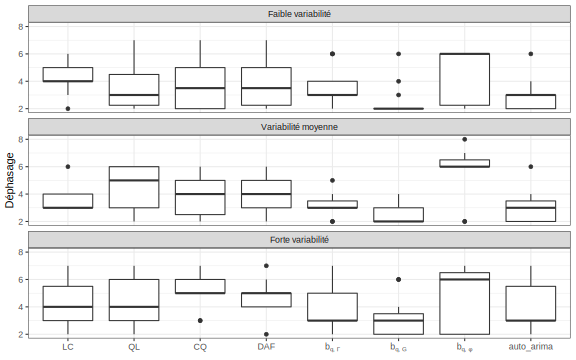
\includegraphics[width=1\linewidth]{img/simulations/phase_shift_simul} 

}

\caption[Distribution des déphasages sur les séries simulées]{Distribution des déphasages sur les séries simulées.}\label{fig:graphstpsimul}

\footnotesize
\normalsize\end{figure}

\begin{table}[!h]

\caption{\label{tab:simulrev}Moyenne des écarts relatifs des révisions pour les différents filtres sur les séries à variabilité moyenne.}
\centering
\begin{tabular}[t]{ccccccc}
\toprule
Méthode & $q=0$ & $q=1$ & $q=2$ & $q=3$ & $q=4$ & $q=5$\\
\midrule
\addlinespace[0.3em]
\multicolumn{7}{l}{\textbf{$MAE_{fe}(q) = \mathbb E\left[\left|(y_{t|t+q} -  y_{t|last})/y_{t|last}\right|\right]$}}\\
\hspace{1em}LC & 0,21 & 0,10 & 0,03 & 0,03 & 0,03 & 0,01\\
\hspace{1em}QL & 0,33 & 0,10 & 0,04 & 0,04 & 0,03 & 0,01\\
\hspace{1em}CQ & 0,45 & 0,13 & 0,13 & 0,09 & 0,06 & 0,02\\
\hspace{1em}DAF & 0,47 & 0,15 & 0,15 & 0,09 & 0,06 & 0,02\\
\hspace{1em}$b_{q,\Gamma}$ & 0,63 & 0,21 & 0,03 & 0,09 & 0,09 & 0,04\\
\hspace{1em}$b_{q,G}$ & 0,83 & 0,37 & 0,03 & 0,09 & 0,09 & 0,04\\
\hspace{1em}$b_{q,\varphi}$ & 0,31 & 0,11 & 0,03 & 0,05 & 0,07 & 0,09\\
\hspace{1em}ARIMA & 0,22 & 0,10 & 0,03 & 0,03 & 0,03 & 0,01\\
\addlinespace[0.3em]
\multicolumn{7}{l}{\textbf{$MAE_{ce}(q)=\mathbb E\left[
\left|(y_{t|t+q} - y_{t|t+q+1})/y_{t|t+q+1}\right|
\right]$}}\\
\hspace{1em}LC & 0,19 & 0,10 & 0,02 & 0,01 & 0,07 & 0,01\\
\hspace{1em}QL & 0,29 & 3,46 & 0,00 & 0,03 & 0,04 & 0,01\\
\hspace{1em}CQ & 0,43 & 0,02 & 0,10 & 0,07 & 0,05 & 0,02\\
\hspace{1em}DAF & 0,66 & 0,24 & 0,11 & 0,14 & 0,06 & 0,02\\
\hspace{1em}$b_{q,\Gamma}$ & 0,38 & 0,32 & 0,09 & 0,00 & 0,41 & 0,04\\
\hspace{1em}$b_{q,G}$ & 0,70 & 0,46 & 0,10 & 0,00 & 0,43 & 0,04\\
\hspace{1em}$b_{q,\varphi}$ & 0,22 & 0,16 & 0,08 & 0,05 & 0,03 & 0,09\\
\hspace{1em}ARIMA & 0,21 & 0,13 & 0,02 & 0,02 & 0,25 & 0,01\\
\bottomrule
\end{tabular}
\end{table}

Concernant les révisions, la variabilité de la série a peu d'impact sur les performances respectives des différentes méthodes mais joue sur les ordres de grandeurs.
Globalement, les filtres LC minimisent toujours les révisions (voir tableau \ref{tab:simulrev}) et les révisions sont plus importantes avec les filtres CQ, DAF et les filtres RKHS autres que \(b_{q,\varphi}\).
Pour les filtres QL, il y a une forte révision entre la deuxième et la troisième estimation : cela peut venir du fait que pour la deuxième estimation (lorsque l'on connait un point dans le futur), le filtre QL associe un poids plus important à l'estimation en \(t+1\) qu'à l'estimation en \(t\), ce qui crée une discontinuité.
Pour les filtres polynomiaux autres que le filtre LC, les révisions importantes à la première estimation étaient prévisibles au vu de la courbe des coefficients : un poids très important est associé à l'observation courante et il y une forte discontinuité entre la moyenne mobile utilisée pour l'estimation en temps réelle (lorsqu'aucun point dans le futur n'est connu) et les autres moyennes mobiles.

Le prolongement de la série par un modèle ARIMA donnent révisions avec les dernières estimations du même ordre de grandeur que le filtre LC mais des révisions plus importantes entre les estimations consécutives (on pouvait s'y attendre comme souligné dans la section \ref{subec:mmetprev}).

En somme, par rapport au filtre LC, la réduction du déphasage du filtre \(b_{q,G}\) se fait au coût de révisions 4 fois plus importantes lorsque la variabilité de la série est moyenne.
Pour les séries à forte variabilité, les révisions sont du même ordre de grandeur mais l'écart est bien plus important pour les séries à faible variabilité.

\hypertarget{comparaison-avec-lapproche-fst}{%
\subsubsection{Comparaison avec l'approche FST}\label{comparaison-avec-lapproche-fst}}

Pour le choix des poids dans l'approche FST, l'idée retenue dans cette étude est de faire un quadrillage du plan \([0,1]^3\) avec un pas de 0,05 et en imposant \(\alpha + \beta + \gamma = 1\)\footnote{
  Comme il n'est pas possible d'avoir un poids associé à la \emph{timeliness} (\(\gamma\)) égale à 1 (sinon la fonction objectif n'est pas strictement convexe), on construit également un filtre avec un poids très proche de 1 (\(1-1/1000\)).}.
Pour chaque combinaison de poids, quatre ensembles de moyennes mobiles sont construits en forçant dans la minimisation la préservation de polynômes de degré 0 à 3.
Le filtre symétrique utilisé est toujours celui de Henderson.
Ces différentes moyennes mobiles sont ensuite comparées relativement aux performances des filtres LC et, par simplification, uniquement sur les séries simulées à variabilité moyenne.

\begin{figure}

{\centering 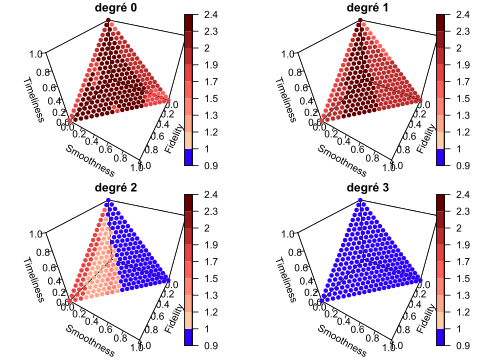
\includegraphics[width=0.9\linewidth]{img/simulations/fst_mediumvariability_tp_med} 

}

\caption[Médiane du déphasage relatif des filtres FST par rapport au filtre LC selon les poids sur les séries simulées à variabilité moyenne]{Médiane du déphasage relatif des filtres FST par rapport au filtre LC selon les poids sur les séries simulées à variabilité moyenne.}\label{fig:graphstpsimulfst}

\footnotesize
\normalsize\end{figure}

En termes de déphasage, en médiane, les filtres qui sont plus performants que les filtres LC sont ceux qui préservent le polynômes de degré 2 et ayant un poids associé à la \emph{fidelity} (\(\beta\)) inférieur à 0,5 et ceux qui préservent les polynômes de degré 3 (figure \ref{fig:graphstpsimulfst}).
En revanche, une analyse plus fine des résultats montre qu'en moyenne le déphasage est plus élevé qu'avec la méthode LC pour tous les filtres FST mais les résultats sont quasiment équivalents (entre 1,0 et 1,1) pour les filtres qui préservent les polynômes de degré 2 avec \(\alpha = \beta =0,05\) et \(\alpha = 0,05, \, \beta =0\) et ceux qui préservent les polynômes de degré 3 avec \(\beta=0\).

\begin{figure}

{\centering 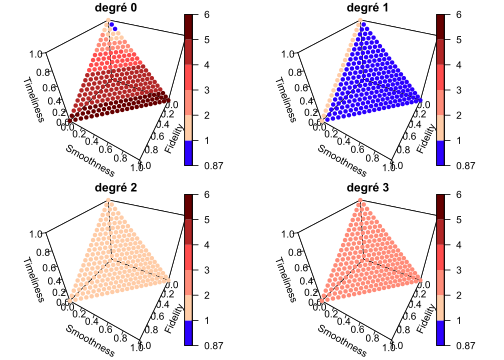
\includegraphics[width=0.9\linewidth]{img/simulations/fst_mediumvariability_fe_q0} 

}

\caption[Moyenne des écarts relatifs des révisions entre la première et la dernière estimation (\(MAE_{fe}(0)\)), comparativement aux révisions du filtre LC sur les séries à variabilité moyenne]{Moyenne des écarts relatifs des révisions entre la première et la dernière estimation (\(MAE_{fe}(0)\)), comparativement aux révisions du filtre LC sur les séries à variabilité moyenne.}\label{fig:graphsfeq0simulfst}

\footnotesize
\normalsize\end{figure}

\begin{figure}

{\centering 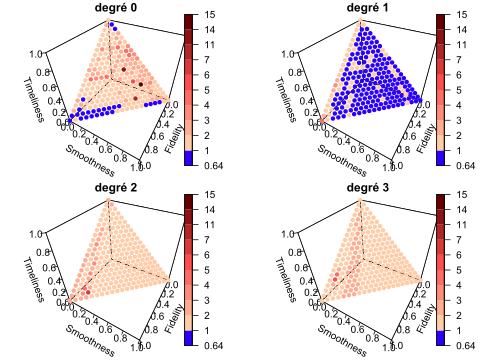
\includegraphics[width=0.9\linewidth]{img/simulations/fst_mediumvariability_ceq0} 

}

\caption[Moyenne des écarts relatifs des révisions entre la première et la deuxième estimation (\(MAE_{ce}(0)\)), comparativement aux révisions du filtre LC sur les séries à variabilité moyenne]{Moyenne des écarts relatifs des révisions entre la première et la deuxième estimation (\(MAE_{ce}(0)\)), comparativement aux révisions du filtre LC sur les séries à variabilité moyenne.}\label{fig:graphsceq0simulfst}

\footnotesize
\normalsize\end{figure}

En termes de révisions (figures \ref{fig:graphsfeq0simulfst} et \ref{fig:graphsceq0simulfst}), les révisions entre la première et dernière estimation et entre la première et deuxième estimation sont inférieures à celles du filtre LC lorsque les filtres préservent les polynômes de degré 1. En revanche, avec les filtres qui préserve les polynômes de degré 3 les révisions entre la première et dernière estimation sont en moyenne plus de deux fois plus importante qu'avec le filtre LC et sont modérément plus élevées (rapport entre 1 et 2).

En somme, même si une étude plus approfondie devrait être menée, pour l'étude de la méthode FST il parait opportun de se concentrer sur les filtres qui préserve les polynômes de degré 2 avec un poids associé au critère \emph{fidelity} élevé et un poids faible associé au critère \emph{smoothness}.

\hypertarget{suxe9rie-ruxe9elle}{%
\subsection{Série réelle}\label{suxe9rie-ruxe9elle}}

Les différentes méthodes sont également comparées sur le point de retournement d'avril 2020 sur les ventes au détail des États-Unis (série \texttt{RETAILx} de la base FRED-MD \textcite{fredmd}, utilisée en logarithme).
C'est une série avec une variabilité moyenne.
Les résultats des différentes estimations sont tracées dans les figures \ref{fig:retailxlp} à \ref{fig:retailxfst2}.
Pour l'approche FST, on ne retient que les filtres obtenus avec les poids \(\begin{pmatrix}\alpha&\beta&\gamma\end{pmatrix} = \begin{pmatrix}0,05 &0,00&0,95\end{pmatrix},\, \begin{pmatrix}0,00 &0,05&0,95\end{pmatrix},\, \begin{pmatrix}0,05 &0,05&0,90\end{pmatrix}\) ou \(\begin{pmatrix}0 &0&1\end{pmatrix}\) et en préservant les tendances de degré 2 ou 3.

\begin{figure}

{\centering 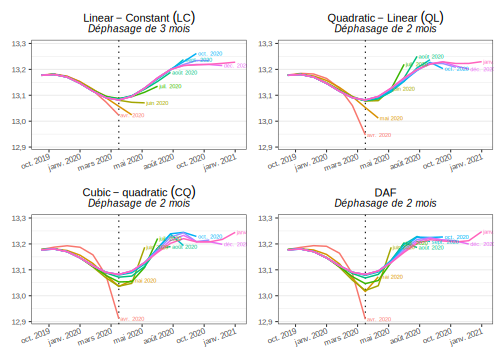
\includegraphics[width=0.9\linewidth]{img/nber/retailx_lp} 

}

\caption[Estimations successives de la tendance-cycle des ventes au détail aux États-Unis avec les méthodes polynomiales locales]{Estimations successives de la tendance-cycle des ventes au détail aux États-Unis avec les méthodes polynomiales locales.}\label{fig:retailxlp}

\footnotesize
\normalsize\end{figure}

\begin{figure}

{\centering 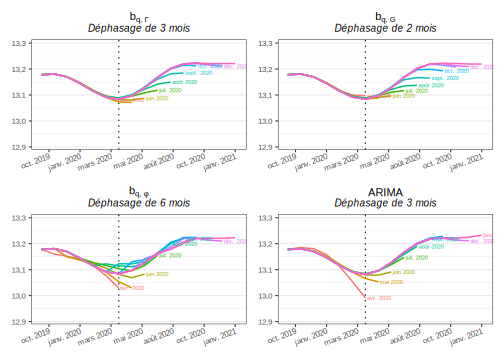
\includegraphics[width=0.9\linewidth]{img/nber/retailx_rkhs_arima} 

}

\caption[Estimations successives de la tendance-cycle des ventes au détail aux États-Unis avec les RKHS et en prolongeant la série par modèle ARIMA]{Estimations successives de la tendance-cycle des ventes au détail aux États-Unis avec les RKHS et en prolongeant la série par modèle ARIMA.}\label{fig:retailxrkhs}

\footnotesize
\normalsize\end{figure}

\begin{figure}

{\centering 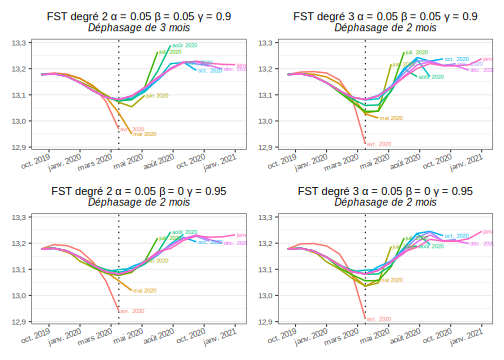
\includegraphics[width=0.9\linewidth]{img/nber/retailx_fstp1} 

}

\caption[Estimations successives de la tendance-cycle des ventes au détail aux États-Unis avec la méthode FST et \(\begin{pmatrix}\alpha&\beta&\gamma\end{pmatrix} = \begin{pmatrix}0,05 &0,00&0,95\end{pmatrix}\) ou \(\begin{pmatrix}0,05 &0,05&0,90\end{pmatrix}\)]{Estimations successives de la tendance-cycle des ventes au détail aux États-Unis avec la méthode FST et \(\begin{pmatrix}\alpha&\beta&\gamma\end{pmatrix} = \begin{pmatrix}0,05 &0,00&0,95\end{pmatrix}\) ou \(\begin{pmatrix}0,05 &0,05&0,90\end{pmatrix}\).}\label{fig:retailxfst1}

\footnotesize
\normalsize\end{figure}

\begin{figure}

{\centering 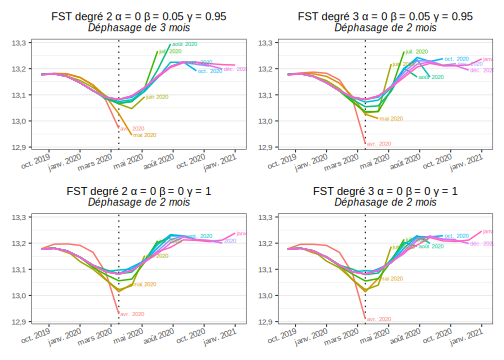
\includegraphics[width=0.9\linewidth]{img/nber/retailx_fstp2} 

}

\caption[Estimations successives de la tendance-cycle des ventes au détail aux États-Unis avec la méthode FST et \(\begin{pmatrix}\alpha&\beta&\gamma\end{pmatrix} =\begin{pmatrix}0,00 &0,05&0,95\end{pmatrix}\) ou \(\begin{pmatrix}0 &0&1\end{pmatrix}\)]{Estimations successives de la tendance-cycle des ventes au détail aux États-Unis avec la méthode FST et \(\begin{pmatrix}\alpha&\beta&\gamma\end{pmatrix} =\begin{pmatrix}0,00 &0,05&0,95\end{pmatrix}\) ou \(\begin{pmatrix}0 &0&1\end{pmatrix}\).}\label{fig:retailxfst2}

\footnotesize
\normalsize\end{figure}

Même si presque toutes les méthodes ont un déphasage d'au plus 3 mois sur ce point de retournement, les estimations intermédiaires différent grandement.
Il y a par exemple nettement plus de variabilités dans les estimations en temps réel pour les méthode QL, CQ et DAF et les filtres FST (figures \ref{fig:retailxlp}, \ref{fig:retailxfst1} et \ref{fig:retailxfst2}), avec des estimations intermédiaires qui semblent peu plausibles (notamment pour la première estimation du mois d'avril 2020). Les premières estimations avec le filtre LC ne capte pas la remontée en mai et juin 2020 : cela peut provenir du fait qu'en fin de série, la tendance modélisée est linéaire.
Concernant les filtres RKHS, les estimations intermédiaires du filtre \(b_{q,\varphi}\) semblent très erratiques, ce qui s'explique par le fait que les moyennes mobiles asymétriques utilisées lorsque l'on se rapproche du cas symétrique sont éloignées de la moyenne mobile symétrique d'Henderson.
En revanche, les filtres \(b_{q,\Gamma}\) et \(b_{q,G}\) donnent des estimations intermédiaires proches de l'estimation finale, tout en minimisant le déphasage.

La qualité des estimations intermédiaires peut également être analysée grâces aux prévisions implicites des différentes méthodes. Pour rappel, il s'agit des prévisions de la série brute qui, en appliquant le filtre symétrique de Henderson sur la série prolongée, donne les mêmes estimations que les moyennes mobiles asymétriques. L'annexe \ref{an-implicitforecasts} rassemble les différentes prévisions implicites des filtres étudiés dans cette section.
Les prévisions implicites des filtres polynomiaux autres que LC, des filtres FST et du filtre \(b_{q,\varphi}\) sont très peu plausibles et très éloignés des valeurs futures.
Le contrecoup en mai 2020 suite à la baisse d'avril 2020 ne sont pas prévus par le modèle ARIMA mais le sont par les filtres LC et RKHS, en revanche, les prévisions à l'horizon de 6 mois peuvent être assez éloignées des valeurs attendues.

\newpage

\hypertarget{conclusion}{%
\section*{Conclusion}\label{conclusion}}
\addcontentsline{toc}{section}{Conclusion}

Pour l'analyse conjoncturel, la majorité des statisticiens fait directement ou indirectement appel à des méthodes d'extraction de la tendance-cycle.
Elles sont par exemple utilisées pour réduire le bruit d'un indicateur afin d'en améliorer son analyse, et les modèles utilisées (comme les modèles de prévision) utilisent généralement sur des séries désaisonnalisées qui s'appuient sur ces méthodes.

Cette étude fait une première revue de la littérature des méthodes de construction des filtres asymétriques pour l'extraction de la tendance-cycle, utilisées pour l'estimation en temps réel (i.e., l'estimation des derniers points connus).
Toutes ces méthodes peuvent se voir comme des cas particuliers d'une théorie générale de construction des moyennes mobiles.
Elles sont par ailleurs facilement mobilisables et comparables grâce au \emph{package} \faIcon{r-project} \texttt{rjdfilters}.
Celui-ci permet d'utiliser plusieurs outils, comme la construction des prévisions implicites, qui peuvent aider les statisticiens à évaluer la qualité des estimations récentes des différents filtres.

La comparaison des différentes méthodes, bien que perfectible, permet de tirer quelques enseignements pour la construction de ces moyennes mobiles.
Premièrement, en fin de période, chercher à conserver des tendances polynomiales de degré supérieur à un (filtres QL, CQ et DAF et certains filtres FST) semble introduire de la variance dans les estimations (et donc plus de révisions) sans gain significatif en termes de détection de point de retournement.
Il faut en revanche que la longueur du filtre utilisé soit adapté à la variabilité de la série : si le filtre utilisé est trop long (c'est-à-dire si la variabilité de la série est «~moyenne~»), conserver des tendances polynomiale de degré au plus 1 (méthode LC) produit de moins bons résultats en termes de détection des points de retournement.

Deuxièmement, la théorie des RKHS semble permettre la construction de filtres qui pourraient donner un bon compromis entre minimisation du déphasage et révisions (filtre \(b_{q,G}\)).
Toutefois, leur calibration peut être sujette à des problèmes d'optimisation et conduire à des estimations intermédiaires erratiques (filtre \(b_{q,\varphi}\)).

Enfin, la moins bonne performance apparente de certains filtres basés sur l'approche FST ou les RKHS pourrait provenir de l'utilisation de filtres sous-optimaux lorsque que l'on s'approche du cas d'utilisation du filtre symétrique.
Sur l'approche FST par exemple, rien ne justifie que l'on devrait utiliser les mêmes poids entre fidélité, lissage et temporalité pour la construction de toutes les moyennes mobiles asymétriques.
Plus d'études devraient être faites pour savoir si, pour la construction des filtres asymétriques minimisant le déphasage, on pourrait se concentrer uniquement sur les ceux utilisés lorsque peu d'observations futures sont disponibles.
Cela impliquerait notamment de revoir la méthodologie et les indicateurs utilisés.

Cette étude pourrait être étendue de plusieurs manières.

Tout d'abord, elle n'est pas exhaustive et pourrait donc être complétée.\\
Parmi les approches étudiées, l'extension proposée aux méthodes polynomiales locales afin d'ajouter un critère sur le déphasage pourrait donner des résultats prometteurs.
Sur les méthodes FST et DAF, des méthodes de réduction de dimension pourraient être mobilisées afin d'étudier les paramètres les plus déterminants sur les performances des filtres.\\
Parmi les approches récentes non étudiées, nous pouvons citer \textcite{vasyechko2014new} qui utilisent le noyau d'Epanechnikov pour construire des filtres asymétriques de 13 termes (i.e., en utilisant un nombre de points dans le passé différent du filtre symétrique), et \textcite{FengSchafer2021} qui proposent, en fin de période, l'utilisation de poids optimaux (au sens de l'erreur quadratique moyenne) dans les régressions polynomiales locales.

Parmi les pistes d'extension, on pourrait s'intéresser à l'impact de la longueur des filtres dans la détection des points de retournement.
En effet, les filtres asymétriques sont calibrés avec des indicateurs calculés pour l'estimation des filtres symétriques (par exemple pour déterminer automatiquement sa longueur), alors qu'une estimation locale pourrait être préférée.
Par ailleurs, nous nous sommes concentrés uniquement sur les séries mensuelles dont le filtre symétrique est de 13 termes, mais les résultats peuvent être différents si le filtre symétrique étudié est plus long/court et si l'on étudie des séries à d'autres fréquences (trimestrielles ou journalières par exemple).

Une autre piste pourrait être d'étudier l'impact des points atypiques : les moyennes mobiles, comme tout opérateur linéaire, sont très sensibles à la présence des points atypiques.
Pour limiter leur impact, dans X-13ARIMA une forte correction des points atypiques est effectuée sur la composante irrégulière avant d'appliquer les filtres pour extraire la tendance-cycle.
Cela amène donc à étudier l'impact de ces points sur l'estimation de la tendance-cycle et des points de retournement, mais aussi à explorer de nouveaux types de filtres asymétriques basés sur des méthodes robustes (comme les régressions locales robustes ou les médianes mobiles).

\newpage

\hypertarget{appendix-annexe}{%
\appendix}


\newpage

\hypertarget{an-diag}{%
\section{Synthèse des liens entre les différentes méthodes de construction de moyennes mobiles}\label{an-diag}}

\begin{figure}[!ht]

{\centering 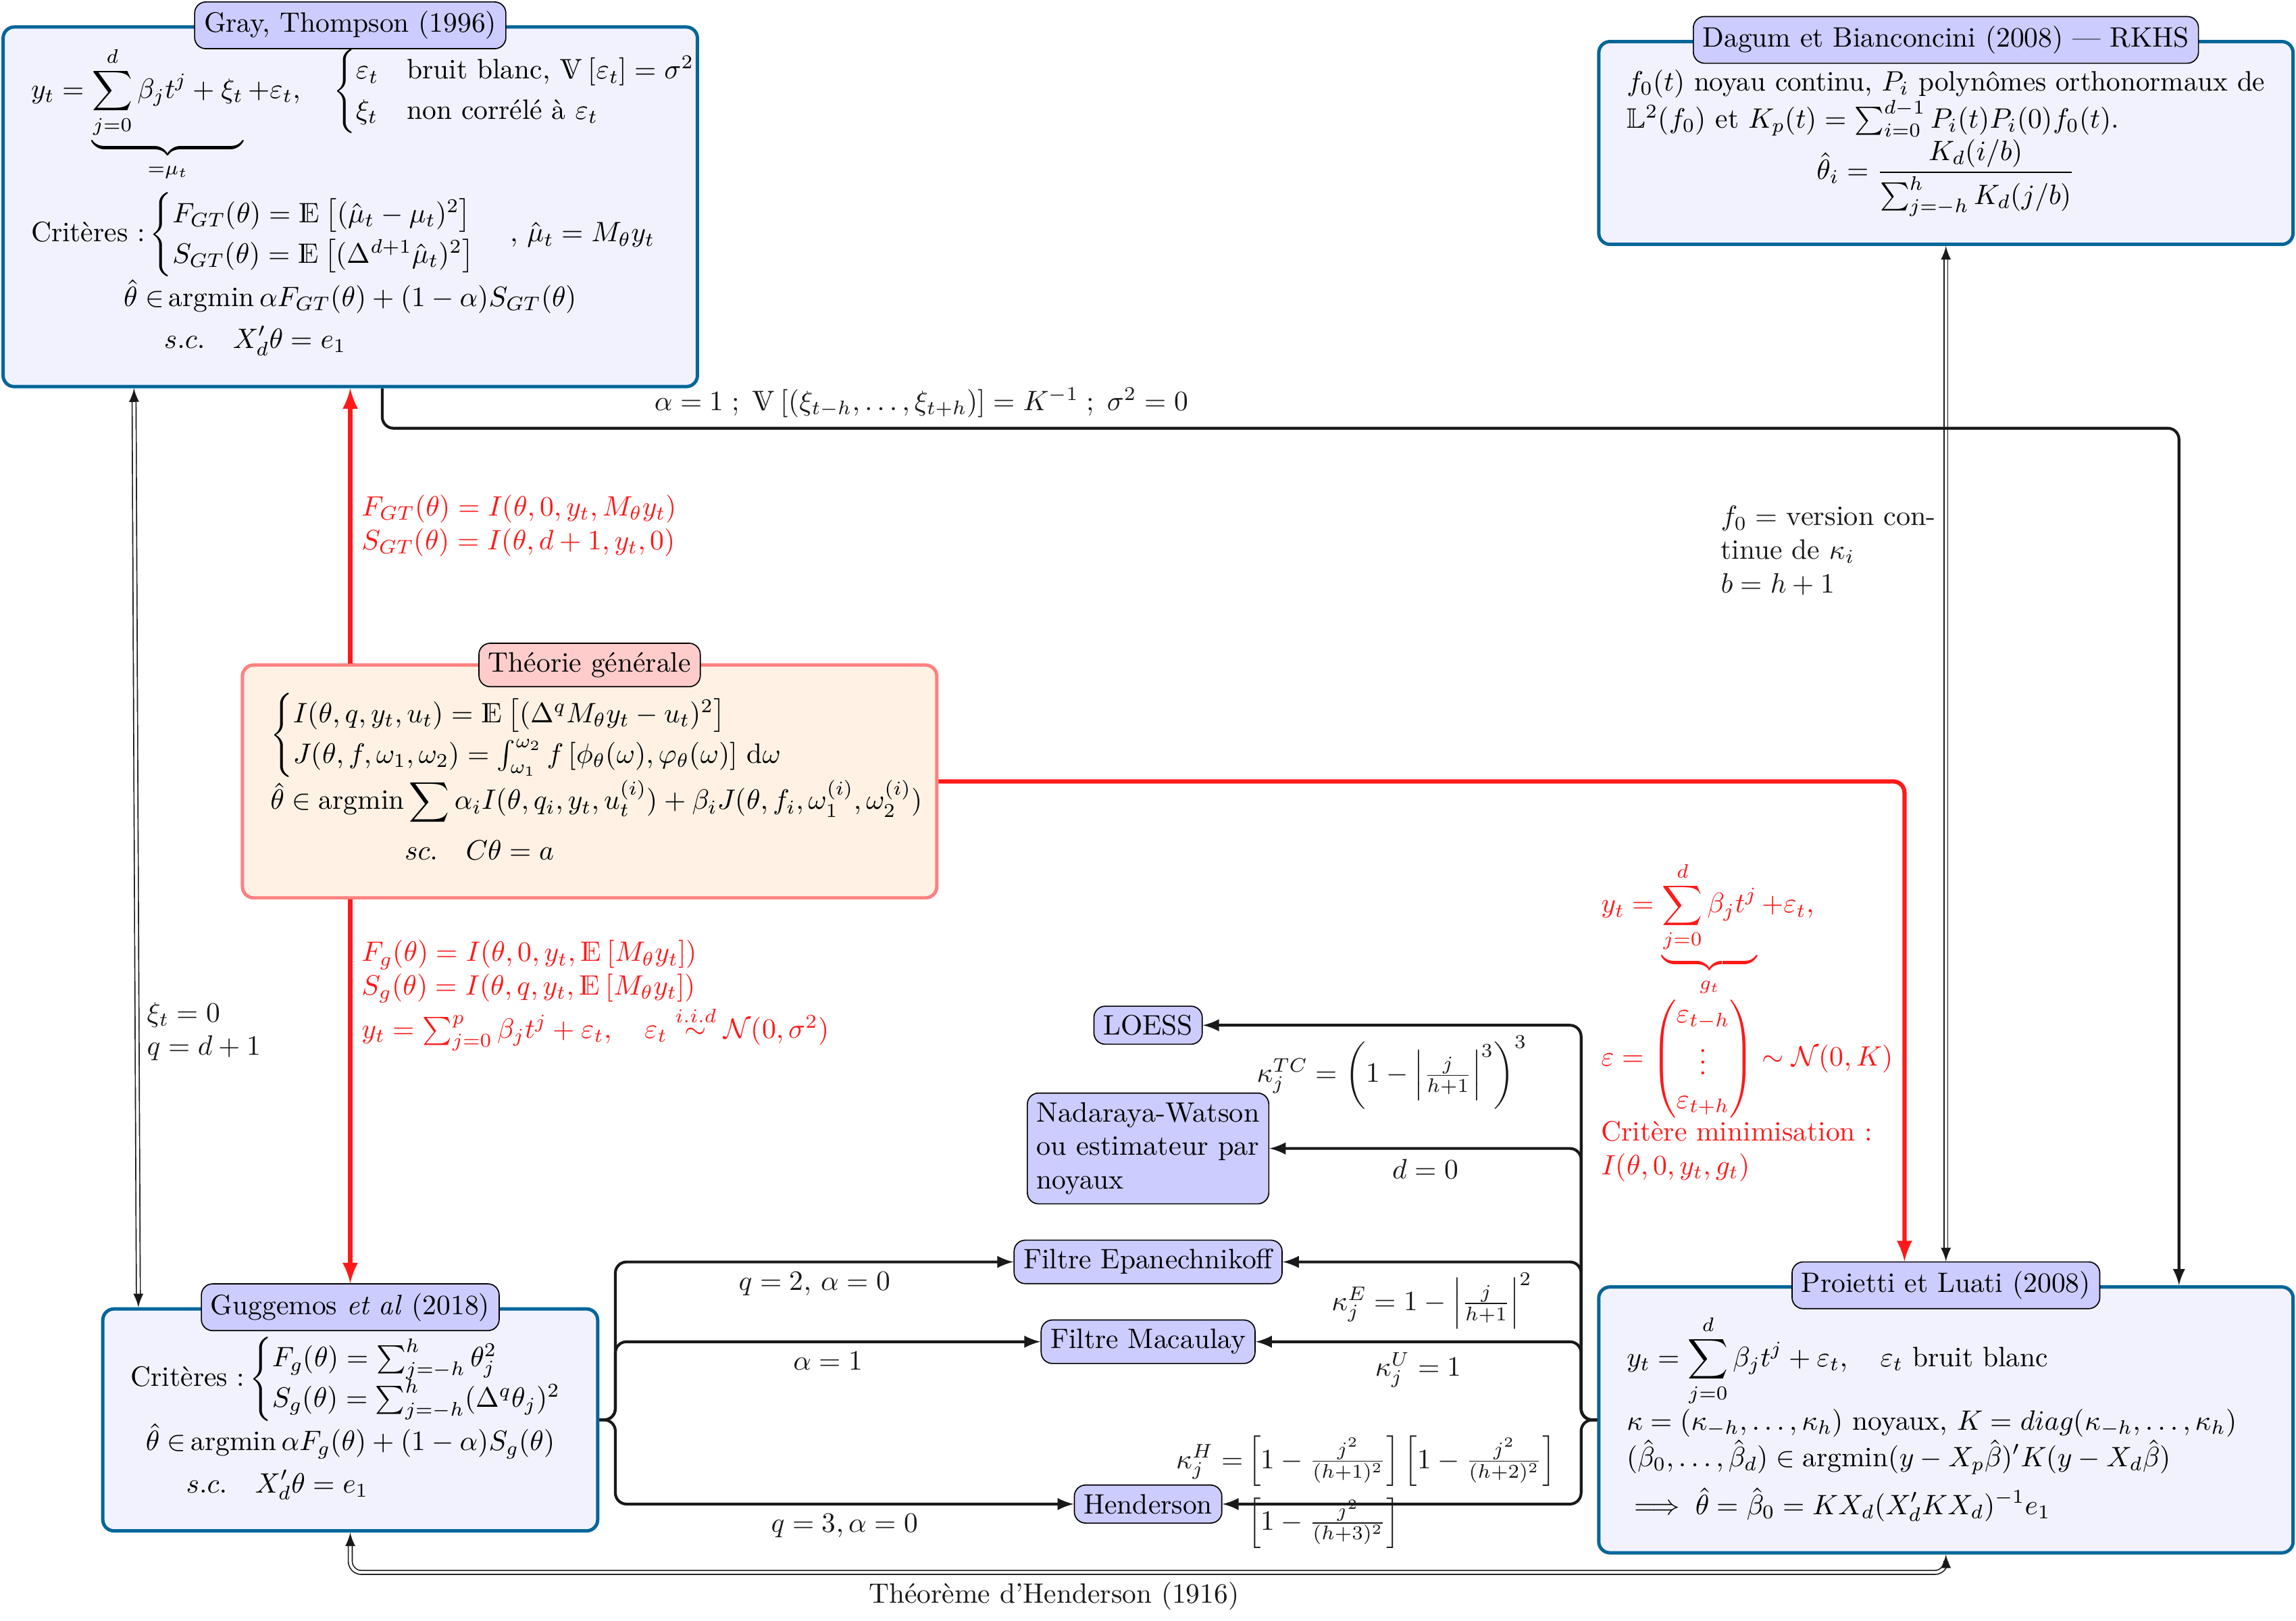
\includegraphics[width=0.8\textheight,angle=90]{img/bookdown/pdf/diag-gen-sym-1} 

}

\caption[Synthèse des méthodes de construction de moyennes mobiles symétriques \(\theta=(\theta_{-h},\dots,\theta_{h})\) de \(2h+1\) termes]{Synthèse des méthodes de construction de moyennes mobiles symétriques \(\theta=(\theta_{-h},\dots,\theta_{h})\) de \(2h+1\) termes.}\label{fig:diag-gen-sym}

\footnotesize


\emph{Note de lecture} : \emph{\(X = X_d = \begin{pmatrix} x_0 \quad\cdots \quad x_d \end{pmatrix}\) avec \(x_i'=\begin{pmatrix} (-h)^i \quad \cdots \quad (h)^i\end{pmatrix}\).}
\normalsize\end{figure}

\begin{figure}[!ht]

{\centering 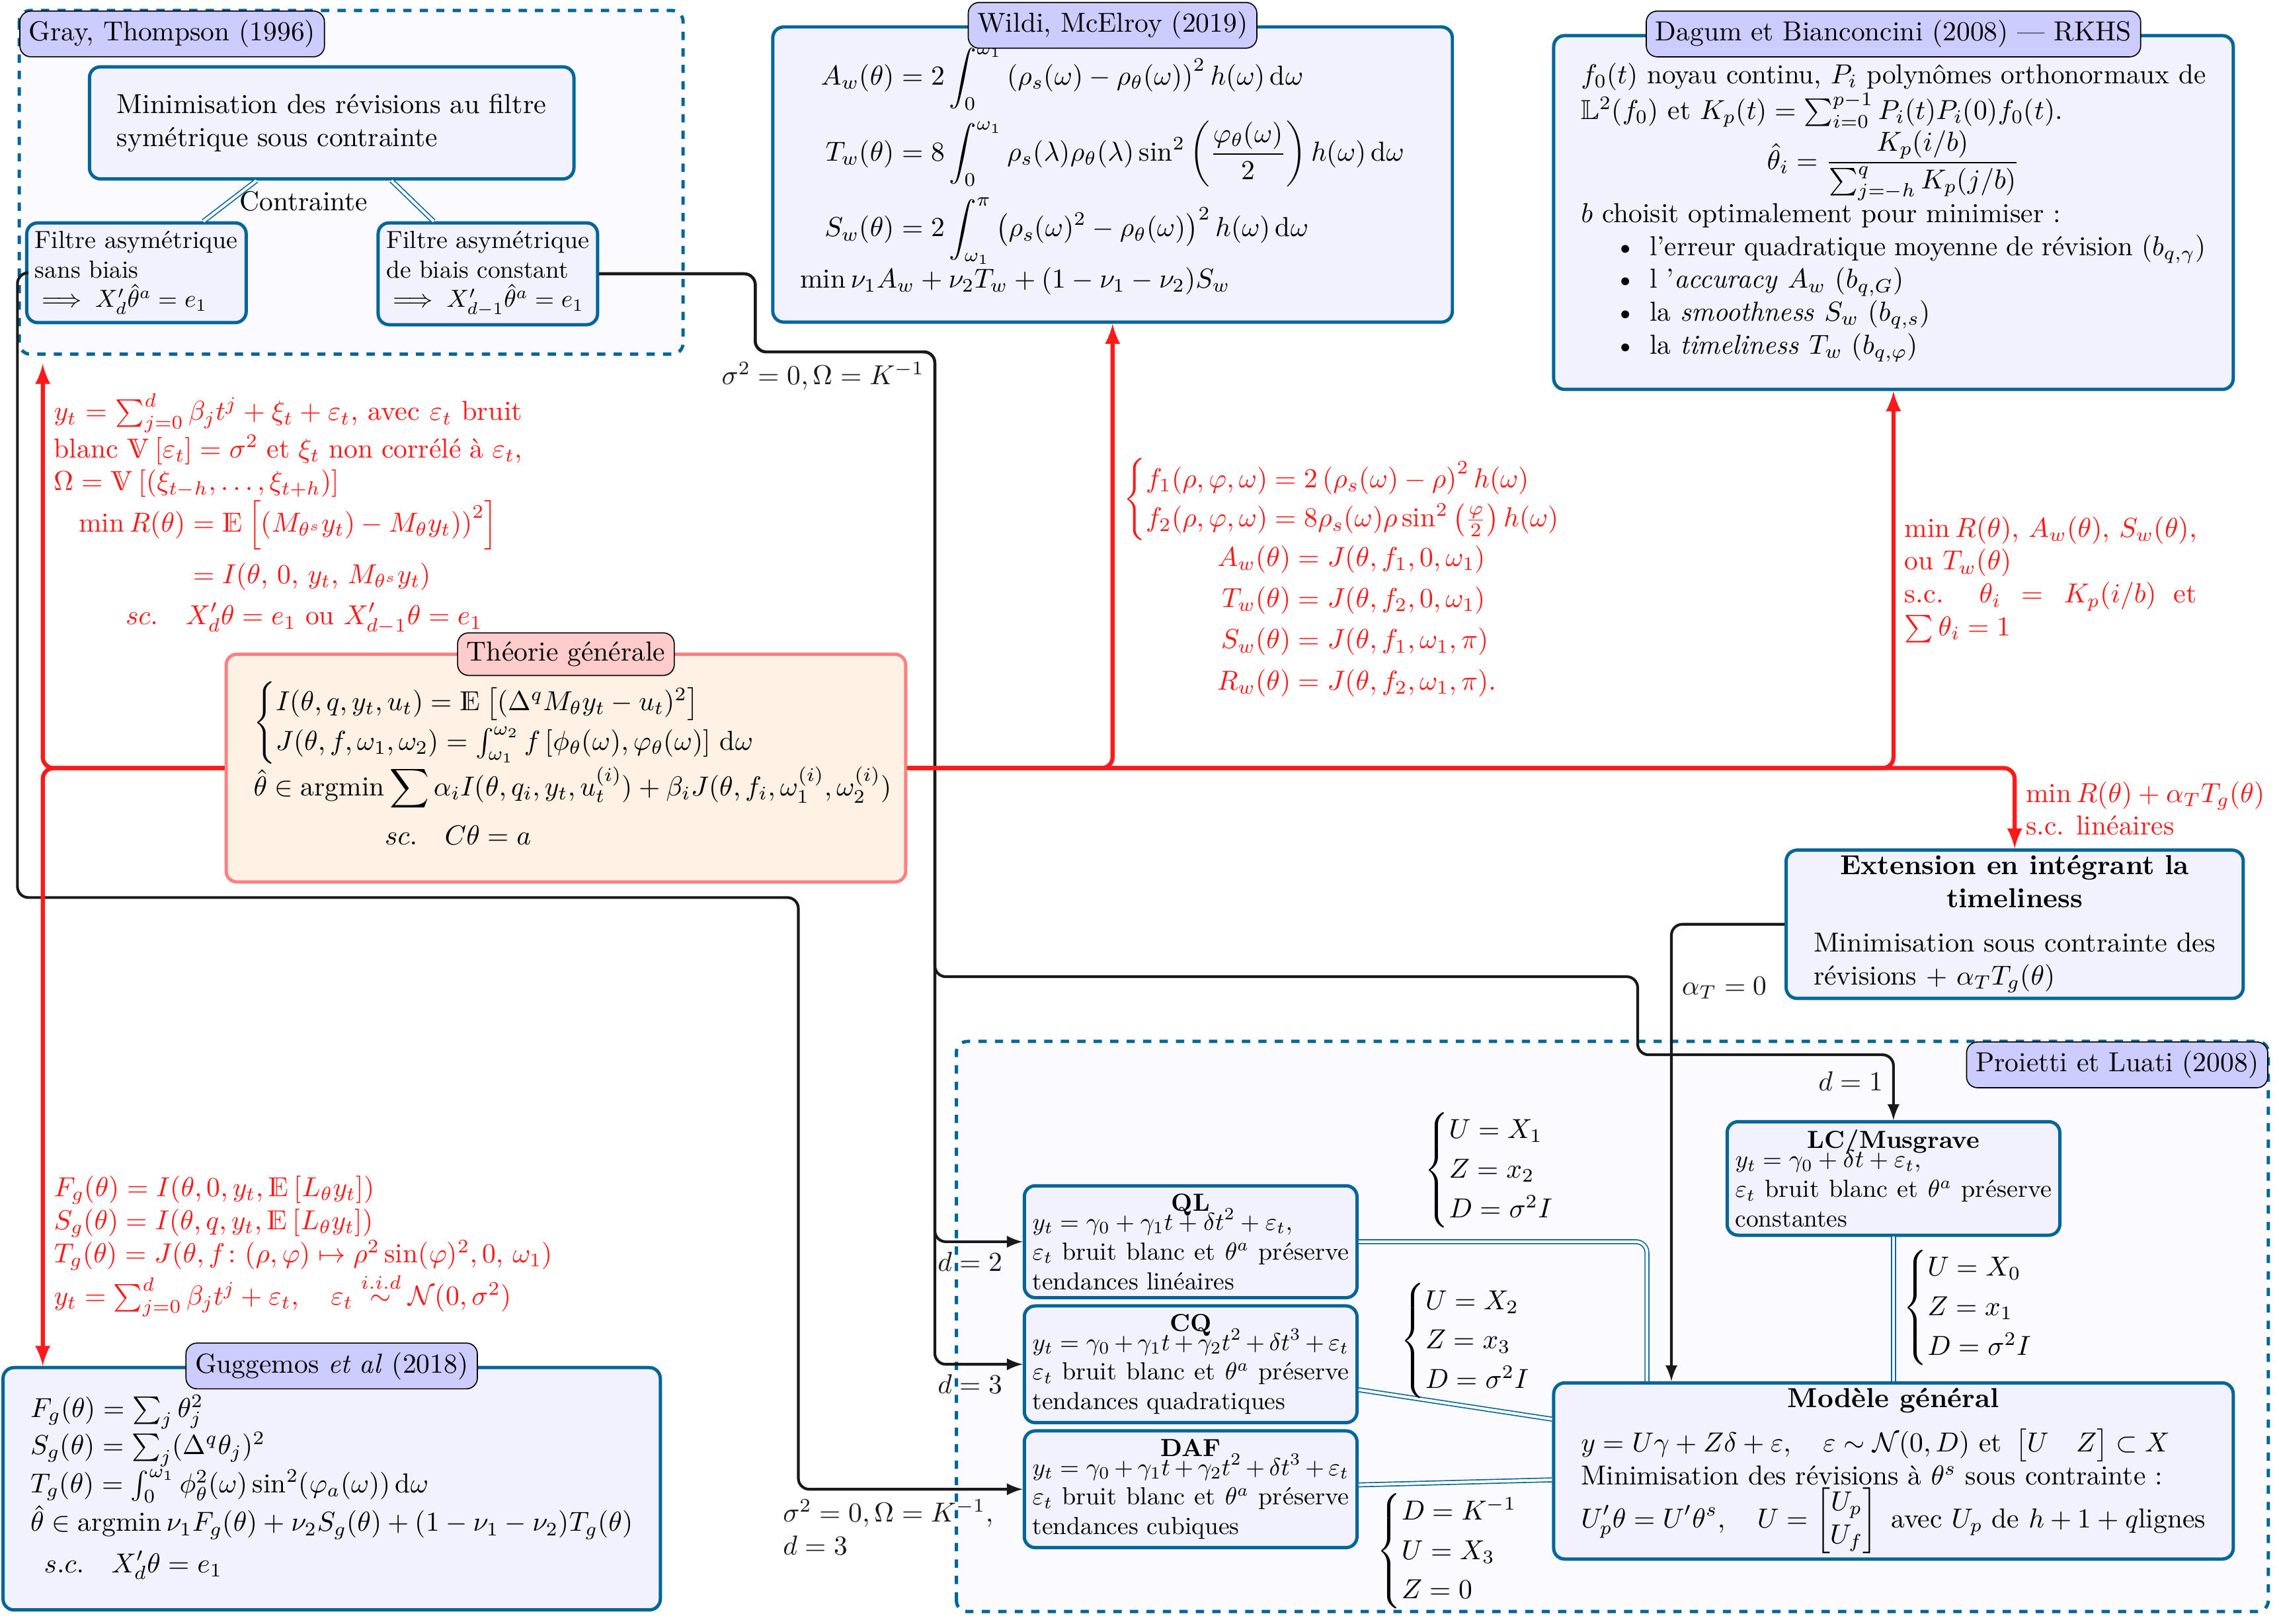
\includegraphics[width=0.8\textheight,angle=90]{img/bookdown/pdf/diag-gen-asym-1} 

}

\caption[Synthèse des méthodes de construction de moyennes mobiles asymétriques \(\theta=(\theta_{-h},\dots,\theta_{q})\), \(0\leq q< h\) avec \(\theta^s\) le filtre symétrique de référence de \(2h+1\) termes]{Synthèse des méthodes de construction de moyennes mobiles asymétriques \(\theta=(\theta_{-h},\dots,\theta_{q})\), \(0\leq q< h\) avec \(\theta^s\) le filtre symétrique de référence de \(2h+1\) termes.}\label{fig:diag-gen-asym}

\footnotesize


\emph{Note de lecture} : \emph{\(X_d = \begin{pmatrix} x_0 \quad\cdots \quad x_d \end{pmatrix}\) avec \(x_i'=\begin{pmatrix} (-h)^i \quad \cdots \quad (q)^i\end{pmatrix}\) et \(X=X_d\) avec \(q=h\).}
\normalsize\end{figure}

\newpage

\hypertarget{an-graphs}{%
\section{Coefficients, fonctions de gain et de déphasage}\label{an-graphs}}

\begin{figure}[H]

{\centering 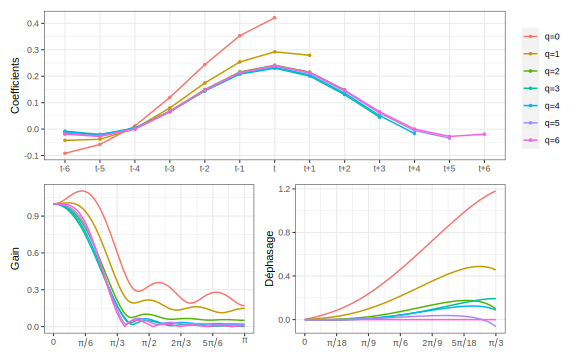
\includegraphics[width=1\linewidth]{img/filters_used/lc} 

}

\caption[Coefficients, fonctions de gain et de déphasage pour le filtre \emph{Linear-Constant} (LC) avec \(I/C=3,5\)]{Coefficients, fonctions de gain et de déphasage pour le filtre \emph{Linear-Constant} (LC) avec \(I/C=3,5\).}\label{fig:graphslc}

\footnotesize
\normalsize\end{figure}

\begin{figure}[H]

{\centering 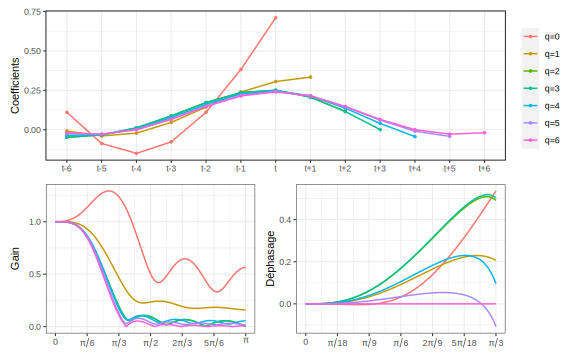
\includegraphics[width=1\linewidth]{img/filters_used/ql} 

}

\caption[Coefficients, fonctions de gain et de déphasage pour le filtre \emph{Quadratic-Linear} (QL) avec \(I/C=3,5\)]{Coefficients, fonctions de gain et de déphasage pour le filtre \emph{Quadratic-Linear} (QL) avec \(I/C=3,5\).}\label{fig:graphsql}

\footnotesize
\normalsize\end{figure}

\begin{figure}[H]

{\centering 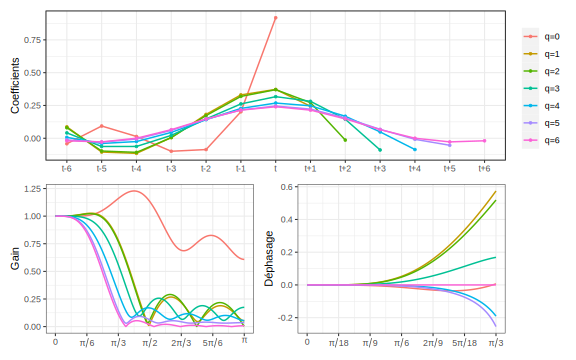
\includegraphics[width=1\linewidth]{img/filters_used/cq} 

}

\caption[Coefficients, fonctions de gain et de déphasage pour le filtre \emph{Cubic-Quadratic} (QL) avec \(I/C=3,5\)]{Coefficients, fonctions de gain et de déphasage pour le filtre \emph{Cubic-Quadratic} (QL) avec \(I/C=3,5\).}\label{fig:graphscq}

\footnotesize
\normalsize\end{figure}

\begin{figure}[H]

{\centering 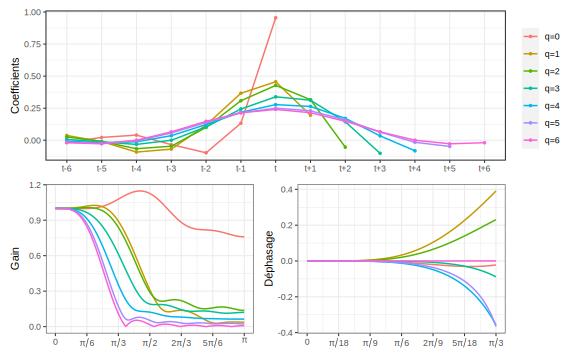
\includegraphics[width=1\linewidth]{img/filters_used/daf} 

}

\caption[Coefficients, fonctions de gain et de déphasage pour le filtre asymétrique direct (DAF) avec \(I/C=3,5\)]{Coefficients, fonctions de gain et de déphasage pour le filtre asymétrique direct (DAF) avec \(I/C=3,5\).}\label{fig:graphsdaf}

\footnotesize
\normalsize\end{figure}

\begin{figure}[H]

{\centering 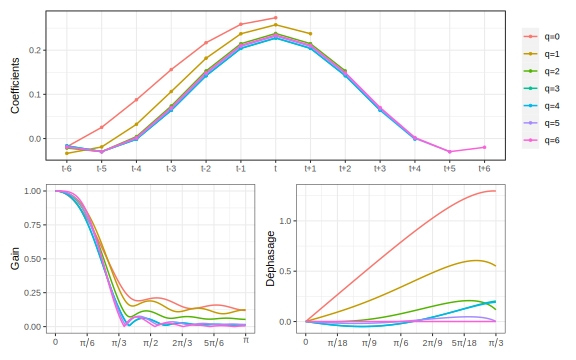
\includegraphics[width=1\linewidth]{img/filters_used/frf} 

}

\caption[Coefficients, fonctions de gain et de déphasage pour le filtre RKHS \(b_{q,\Gamma}\)]{Coefficients, fonctions de gain et de déphasage pour le filtre RKHS \(b_{q,\Gamma}\).}\label{fig:graphsrkhsfrf}

\footnotesize
\normalsize\end{figure}

\begin{figure}[H]

{\centering 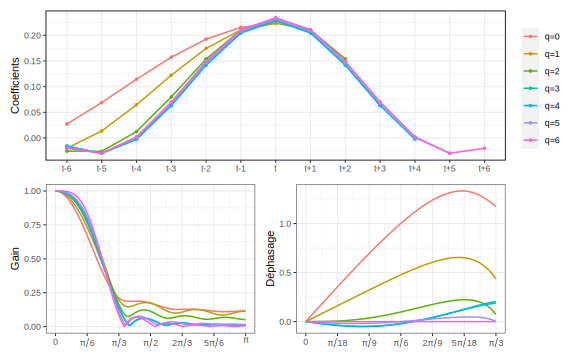
\includegraphics[width=1\linewidth]{img/filters_used/gain} 

}

\caption[Coefficients, fonctions de gain et de déphasage pour le filtre RKHS \(b_{q,G}\)]{Coefficients, fonctions de gain et de déphasage pour le filtre RKHS \(b_{q,G}\).}\label{fig:graphsrkhsgain}

\footnotesize
\normalsize\end{figure}

\begin{figure}[H]

{\centering 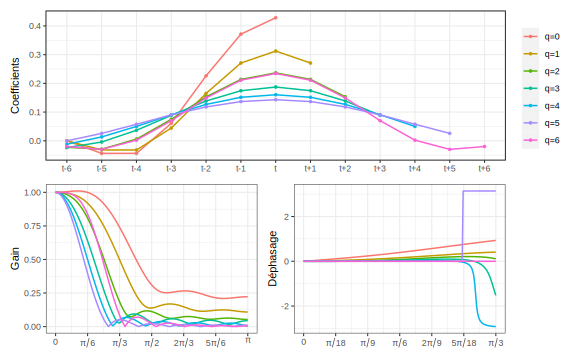
\includegraphics[width=1\linewidth]{img/filters_used/phase} 

}

\caption[Coefficients, fonctions de gain et de déphasage pour le filtre RKHS \(b_{q,\varphi}\)]{Coefficients, fonctions de gain et de déphasage pour le filtre RKHS \(b_{q,\varphi}\).}\label{fig:graphsrkhsphase}

\footnotesize
\normalsize\end{figure}

\newpage

\hypertarget{an-equivfstlp}{%
\section{Équivalence entre l'approche FST et les filtres polynomiaux locaux}\label{an-equivfstlp}}

Dans cette annexe sont tracés les rares poids pour lesquels l'approche FST \textbf{n'est pas} équivalente à l'approche polynomiale locale pour \(h=6\) (filtre symétrique de 13 termes).
Lorsqu'un graphique n'est pas affiché c'est que tous les filtres FST sont équivalents une approche polynomiale locale par moindre carrés pondérés.
Par exemple pour les filtres associés au filtre symétrique de 13 termes (\(h=6\), figure \ref{fig:thhendersonh6}) il n'y a des graphiques que pour les filtres utilisés en temps réel (\(q=0\)) et lorsque ce filtre conserve les constantes (\(d=0\)), les droites (\(d=1\)) et les polynômes de degré 2 (\(d=2\)).
Dans tous les autres cas (i.e., dès que l'on connait au moins un point dans le futur, \(q\geq 1\)), il y a équivalence pour tous les poids testés\footnote{
  Un quadrillage de 200 points de l'intervalle \([0,1]\) a été effectuée et on ne garde que l'ensemble des poids tels que leur somme fasse 1.}.

La \emph{smoothness} est calculée avec le paramètre \(q=3\) (\(S_g(\theta) = \sum_{j}(\nabla^{3}\theta_{j})^{2}\)), comme pour le filtre symétrique d'Henderson.

\begin{figure}[H]

{\centering 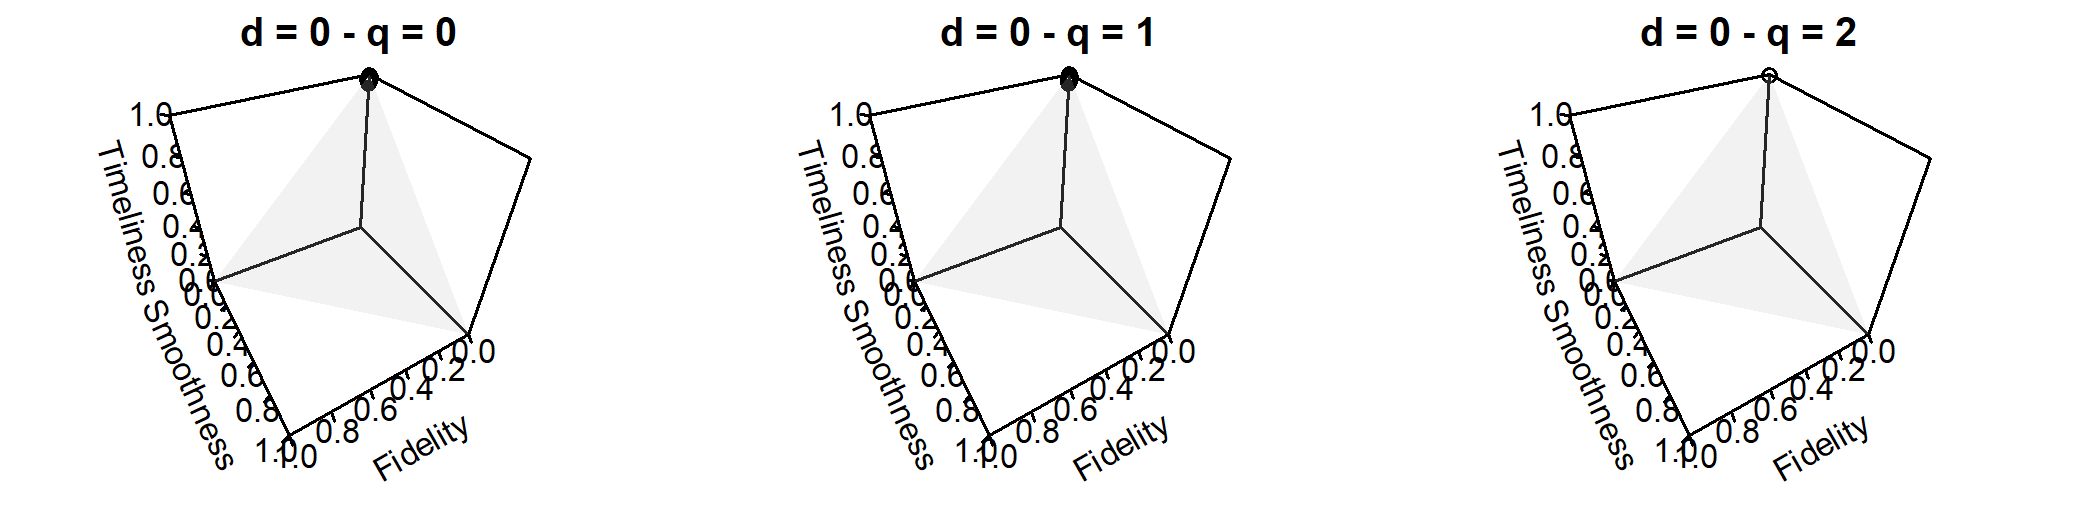
\includegraphics{img/bookdown/pdf/thhendersonh6-1} 

}

\caption[Ensemble des poids pour lesquels la méthode FST n'est pas équivalente aux moindres carrés pondérés pour \(h=6\) (filtre symétrique de 13 termes), sous contrainte de préservation des polynômes de degré au plus 3 (\(d=0,1,2,3\))]{Ensemble des poids pour lesquels la méthode FST n'est pas équivalente aux moindres carrés pondérés pour \(h=6\) (filtre symétrique de 13 termes), sous contrainte de préservation des polynômes de degré au plus 3 (\(d=0,1,2,3\)).}\label{fig:thhendersonh6}

\footnotesize
\normalsize\end{figure}

\newpage

\hypertarget{an-implicitforecasts}{%
\section{\texorpdfstring{Prévisions implicites pour séries \texttt{RETAILx}}{Prévisions implicites pour séries RETAILx}}\label{an-implicitforecasts}}

Cette annexe montre les prévisions implicites associées aux différentes estimations de la tendance-cycle sur les ventes au détail des États-Unis autour du point de retournement d'avril 2020.

\begin{figure}

{\centering 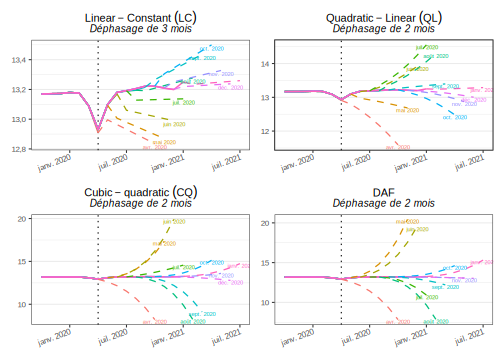
\includegraphics[width=0.9\linewidth]{img/nber/retailx_lp_implicit_forecast} 

}

\caption[Prévisions implicites associées aux estimations successives de la tendance-cycle des ventes au détail aux États-Unis avec les méthodes polynomiales locales]{Prévisions implicites associées aux estimations successives de la tendance-cycle des ventes au détail aux États-Unis avec les méthodes polynomiales locales.}\label{fig:retailxiplp}

\footnotesize
\normalsize\end{figure}

\begin{figure}

{\centering 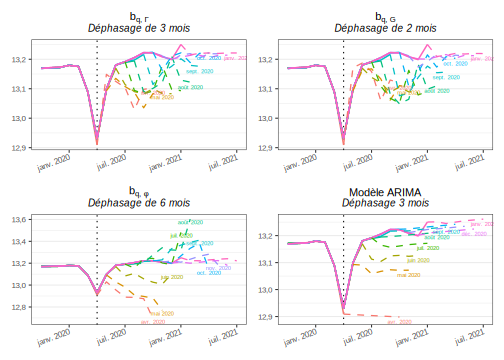
\includegraphics[width=0.9\linewidth]{img/nber/retailx_rkhs_arima_implicit_forecast} 

}

\caption[Prévisions implicites associées aux estimations successives de la tendance-cycle des ventes au détail aux États-Unis avec les RKHS et en prolongeant la série par modèle ARIMA]{Prévisions implicites associées aux estimations successives de la tendance-cycle des ventes au détail aux États-Unis avec les RKHS et en prolongeant la série par modèle ARIMA.}\label{fig:retailxiprkhs}

\footnotesize
\normalsize\end{figure}

\begin{figure}

{\centering 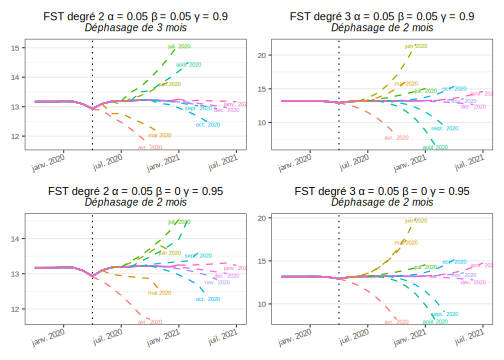
\includegraphics[width=0.9\linewidth]{img/nber/retailx_fstp1_implicit_forecast} 

}

\caption[Prévisions implicites associées aux estimations successives de la tendance-cycle des ventes au détail aux États-Unis avec la méthode FST et \(\begin{pmatrix}\alpha&\beta&\gamma\end{pmatrix} = \begin{pmatrix}0,05 &0,00&0,95\end{pmatrix}\) ou \(\begin{pmatrix}0,05 &0,05&0,90\end{pmatrix}\)]{Prévisions implicites associées aux estimations successives de la tendance-cycle des ventes au détail aux États-Unis avec la méthode FST et \(\begin{pmatrix}\alpha&\beta&\gamma\end{pmatrix} = \begin{pmatrix}0,05 &0,00&0,95\end{pmatrix}\) ou \(\begin{pmatrix}0,05 &0,05&0,90\end{pmatrix}\).}\label{fig:retailxipfst1}

\footnotesize
\normalsize\end{figure}

\begin{figure}

{\centering 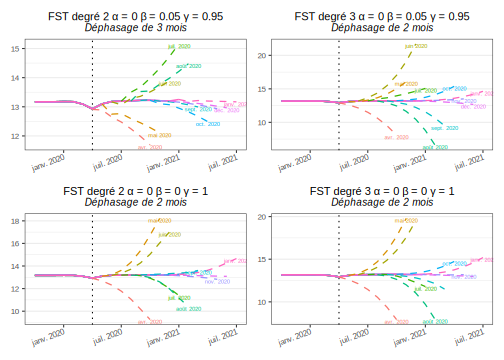
\includegraphics[width=0.9\linewidth]{img/nber/retailx_fstp2_implicit_forecast} 

}

\caption[Prévisions implicites associées aux estimations successives de la tendance-cycle des ventes au détail aux États-Unis avec la méthode FST et \(\begin{pmatrix}\alpha&\beta&\gamma\end{pmatrix} =\begin{pmatrix}0,00 &0,05&0,95\end{pmatrix}\) ou \(\begin{pmatrix}0 &0&1\end{pmatrix}\)]{Prévisions implicites associées aux estimations successives de la tendance-cycle des ventes au détail aux États-Unis avec la méthode FST et \(\begin{pmatrix}\alpha&\beta&\gamma\end{pmatrix} =\begin{pmatrix}0,00 &0,05&0,95\end{pmatrix}\) ou \(\begin{pmatrix}0 &0&1\end{pmatrix}\).}\label{fig:retailxipfst2}

\footnotesize
\normalsize\end{figure}

\newpage

\printbibliography[heading=bibintoc]

\end{document}
